\documentclass[12pt]{article}
\usepackage[top=1in, bottom=1in, left=1in, right=1in]{geometry}
\usepackage{amsfonts}
\usepackage{amsmath}
\usepackage[ngerman,british]{babel}
\usepackage{natbib}
\setcitestyle{aysep={}} %no comma between author and year
\usepackage{url}
\urlstyle{tt}
\usepackage{amssymb}
\usepackage{pdflscape}
\usepackage{placeins} % floatbarrier
\usepackage{subfigure}

\usepackage{array}
\usepackage[flushleft]{threeparttable}
\usepackage{rotating,graphicx}
\usepackage{setspace}
\usepackage{color}
\usepackage{mathtools}
\usepackage[dvipsnames]{xcolor}
\definecolor{CardinalRed}{cmyk}{0,1,0.65,0.34} % Cardinal Red
\usepackage[colorlinks,linkcolor=CardinalRed,citecolor=CardinalRed,urlcolor = CardinalRed]{hyperref}
\usepackage[labelsep=period, font=sc, skip=0pt,justification=centering]{caption}
\usepackage{pdfpages}
\usepackage{framed} % for box around text
\usepackage{titletoc}
\DeclareMathOperator*{\argmax}{arg\,max}
\DeclareMathOperator*{\argmin}{arg\,min}

\usepackage{bm}
\usepackage{bbm}

% change margin for parts
\usepackage{changepage}

% bar on the top hat
\usepackage{accents}

% change spacing above and below an enviornment
\usepackage{etoolbox}
\newcommand{\zerodisplayskips}{%
  \setlength{\abovedisplayskip}{5pt}%
  \setlength{\belowdisplayskip}{5pt}%
  \setlength{\abovedisplayshortskip}{5pt}%
  \setlength{\belowdisplayshortskip}{5pt}}
\appto{\normalsize}{\zerodisplayskips}
\appto{\small}{\zerodisplayskips}
\appto{\footnotesize}{\zerodisplayskips}  
\newcommand{\indep}{\perp \!\!\! \perp}

% no indent for thanks
\usepackage{titling}
\settowidth{\thanksmarkwidth}{*}
\setlength{\thanksmargin}{-\thanksmarkwidth}

% no indent for footnote
\usepackage[flushmargin]{footmisc}
\setlength{\footnotemargin}{2mm}

% dot in section numbering
\usepackage{titlesec}
\titlelabel{\thetitle.\ }
\startcontents[sections]

%% footnotes to endnotes
% \usepackage{endnotes}
% \let\footnote=\endnote
% \usepackage{pa}

%% footnote double spacing
% \renewcommand{\footnotelayout}{\normalsize\doublespacing}
% \setlength{\footnotesep}{\baselineskip} 
% \setlength{\footnotemargin}{2mm}

\usepackage[noend]{algpseudocode}
\usepackage{enumitem}

%%% for DAG ****
\usepackage{tikz}
\usetikzlibrary{positioning,shapes.geometric}

%%% reduce spacing for centering ****
\let\oldcenter\center
\let\oldendcenter\endcenter
\renewenvironment{center}{\setlength\topsep{0pt}\oldcenter}{\oldendcenter}

%\makeatletter
%\def\BState{\State\hskip-\ALG@thistlm}
%\makeatother


\setcounter{MaxMatrixCols}{10}
\providecommand{\U}[1]{\protect \rule{.1in}{.1in}}
%\geometry{verbose,tmargin=2.5cm,bmargin=2.5cm,lmargin=2.45cm,rmargin=2.45cm}
\newtheorem{theorem}{Theorem}
\newtheorem{acknowledgement}[theorem]{Acknowledgement}
\newtheorem{axiom}[theorem]{Axiom}
\newtheorem{case}[theorem]{Case}
\newtheorem{claim}[theorem]{Claim}
\newtheorem{conclusion}[theorem]{Conclusion}
\newtheorem{algorithm}[theorem]{Algorithm}
\newtheorem{condition}[theorem]{Condition}
\newtheorem{conjecture}[theorem]{Conjecture}
\newtheorem{corollary}[theorem]{Corollary}
\newtheorem{criterion}[theorem]{Criterion}
\newtheorem{definition}[theorem]{Definition}
\newtheorem{example}{Example}
\newtheorem{exercise}[theorem]{Exercise}
\newtheorem{lemma}{Lemma}
\newtheorem{notation}[theorem]{Notation}
\newtheorem{problem}[theorem]{Problem}
\newtheorem{proposition}{Proposition}
\newtheorem{Assumption}{Assumption}
\newtheorem{remark}[theorem]{Remark}
\newtheorem{solution}[theorem]{Solution}
\newtheorem{summary}[theorem]{Summary}
\newenvironment{proof}[1][Proof]{\noindent\textbf{#1:} }{\  \rule{0.5em}{0.5em}}
\newcommand{\red}{\textcolor{red}}
\newcommand{\blue}{\textcolor{blue}}
\newcommand{\E}{\mathbb{E}}
\def\T{\mathcal{T}}
\def\C{\mathcal{C}}
\def\ATT{\mathbf{ATT}}
\def\ci{\perp\!\!\!\perp}
\graphicspath{{./graph/}}%
\newcommand{\norm}[1]{\|#1\|} 
\DeclareMathOperator{\tr}{tr}


%%%%%%%%%%%%%%%%%%%%%%%%%%%%%%%%%%%%%%%%%%%%%%%%%%%%%%%%%%
\begin{document}

\onehalfspacing
\date{
  \vspace{-0.5em}\hspace{1.2em}(MIT)\hspace{4.8em}(UNC)\hspace{3.5em}{(Stanford)} \\\vspace{1em}
  First version: 11th July 2019\\
  This version: \today\vspace{2em} 
}


\onehalfspacing
\renewcommand\thesection{\Alph{section}}
\setcounter{page}{1}
\setcounter{table}{0}
\setcounter{figure}{0}
\setcounter{equation}{0}
\setcounter{footnote}{0}
\renewcommand\thetable{A\arabic{table}}
\renewcommand\thefigure{A\arabic{figure}}
%\renewcommand{\thepage}{S-\arabic{page}}
\renewcommand{\theequation}{A\arabic{equation}}
\renewcommand{\thefootnote}{A\arabic{footnote}}


\setcounter{proposition}{0}

\begin{center}
{\Large\bf Supplementary Information \emph{for}}\\\bigskip
{\large\bf A Practical Guide to Counterfactual Estimators for Causal Inference with Time-Series Cross-Sectional Data}\\\bigskip
{\normalsize Licheng Liu (MIT)\hspace{2em}Ye Wang (UNC)\hspace{2em}Yiqing Xu (Stanford)}
\end{center}
\bigskip

% \bigskip\noindent\textbf{{\large -- Not for Publication --}}
\vspace{2em}

\noindent\hspace{0em}{\large\bf \underline{Table of Contents}}

{\bf
\begin{enumerate}\itemsep0ex
    \item[A.] Algorithms and Tests
    \begin{enumerate}\itemsep0ex\vspace{-0.5em}
    	\item[A.1.] The IFEct algorithm
      \item[A.2.] The MC algorithm
    	\item[A.3.] The difference-in-means tests and equivalence tests
      \item[A.4.] Discussion on the no carryover effects assumption
      \item[A.5.] Procedures for the diagnostic tests
	  \end{enumerate}
    \item[B.] Proofs 
    \begin{enumerate}\itemsep0ex\vspace{-0.5em}
      \item[B.1.] Unbiasedness and consistency of FEct and IFEct
      \item[B.2.] FEct as a weighting estimator
    \end{enumerate}
    \item[C.] Inferential Methods
    \item[D.] Additional Monte Carlo Evidence
    \begin{enumerate}\itemsep0ex\vspace{-0.5em}
    \item[D.1.] Describing the data generating processes
    \item[D.2.] IFEct vs MC
    \item[D.3.] $F$ test vs the equivalence test
    \end{enumerate}
    \item[E.] Additional Information on the Empirical Examples
    \begin{enumerate}\itemsep0ex\vspace{-0.5em}
    \item[E.1.] Replicating Hainmueller and Hangartner (2015)
    \item[E.2.] Replicating Fouirnaies and Mutlu-Eren (2015)
    \end{enumerate}    
\end{enumerate}
}
\clearpage

\small



\newpage

\section{Algorithms and Tests}

\subsection{The IFEct Algorithm}\label{sc:algo}

The IFEct algorithm takes for the following four steps. 

\begin{adjustwidth}{20pt}{20pt}

\noindent\textbf{Step 1.} Assuming in round $h$ we have $\hat{\mu}^{(h)}$, 
$\hat{\alpha}_i^{(h)}$, $\hat{\xi}_t^{(h)}$, $ \hat{\lambda}_i^{(h)} $, 
$ \hat{f}_t^{(h)} $ and $ \hat{\beta}^{(h)} $. Denote 
$\dot{Y}_{it}^{(h)} \coloneqq Y_{it} - \hat{\mu}^{(h)} - \hat{\alpha}_i^{(h)} - 
\hat{\xi}_t^{(h)} - \hat{\lambda}_i^{(h)\prime} \hat{f}_t^{(h)} $ 
for the untreated ($ D_{it} = 0 $):

\noindent\textbf{Step 2a.} Update $\hat{\beta}^{(h+1)}$ using the untreated data only (we can set $\hat{\lambda}_{i}^{(0)} = \mathbf{0}$, $\hat{f}_{t}^{(0)} = \mathbf{0}$ in round 0 and run a twoway fixed effects model to initialize $ \mu $, $ \alpha_i $ and $ \xi_t $):
\begin{align*}
  \hat{\beta}^{(h+1)} = 
  \left(\sum_{D_{it} = 0} \mathbf{X}_{it} \mathbf{X}_{it}^{\prime}\right)^{-1}
  \sum_{D_{it} = 0} \mathbf{X}_{it} \dot{Y}_{it}^{(h)}
\end{align*}
Note that matrix $\left(\sum_{D_{it} = 0} \mathbf{X}_{it} \mathbf{X}_{it}^{\prime}\right)^{-1}$ is fixed and does not need to be updated every time.

\noindent\textbf{Step 2b.} For all $i$, $t$, define
\begin{center}
$
W_{it}^{(h+1)} \coloneqq \left\{
\begin{aligned}
& = Y_{it} - \mathbf{X}_{it}^{\prime}\hat{\beta}^{(h+1)}, \ D_{it} = 0 \\
& = \hat{\mu}^{(h)} + \hat{\alpha}_i^{(h)} +
\hat{\xi}_t^{(h)} + \hat{\lambda}_i^{(h)\prime} \hat{f}_t^{(h)}, \ D_{it} = 1
\end{aligned}
\right.
$
\end{center}
For all untreated observations (i.e., $D_{it} = 0$) , calculate $W_{it}^{(h)}$. 
For all treated observations (i.e., $D_{it} = 1$), calculate its conditional expectation:
\begin{center}
   $\E\left(W_{it}^{(h+1)} \big|\hat{\lambda}_{i}^{(h)},\hat{F}_{t}^{(h)}\right) = 
    \hat{\mu}^{(h)} + \hat{\alpha}_i^{(h)} +
\hat{\xi}_t^{(h)} + \hat{\lambda}_{i}^{(h)} \hat{F}_{t}^{(h)}$ 
\end{center}

\noindent\textbf{Step 2c.} Denote 
$ W_{..}^{(h+1)} = \frac{\sum\limits_{i=1}^{N}\sum\limits_{t=1}^{T}W_{it}^{(h+1)}}
{NT} $, 
$ W_{i.}^{(h+1)} = \frac{\sum\limits_{t=1}^{T}W_{it}^{(h+1)}}{T}, \forall i $, 
$ W_{.t}^{(h+1)} = \frac{\sum\limits_{i=1}^{N}W_{it}^{(h+1)}}{N}, \forall t $ and 
$ \tilde{W}_{it}^{(h+1)} = W_{it}^{(h+1)} - W_{i.}^{(h+1)} - W_{.t}^{(h+1)} 
+ W_{..}^{(h+1)} $.  With restrictions: 
$ \sum_{i=1}^{N} \alpha_i = 0 $, $ \sum_{t=1}^{T} \xi_t = 0 $, 
$ \sum_{i=1}^{N} \lambda_i = \mathbf{0} $ and 
$ \sum_{t=1}^{T} f_t = \mathbf{0} $. 


\noindent\textbf{Step 2d.} Update estimates of factors and factor loadings by minimizing the least squares objective function using the complete data of $\mathbf{W}^{(h+1)} = [\tilde{W}_{it}^{(h+1)}]_{\forall i,t}$:
\begin{gather}
  (\hat{\mathbf{F}}^{(h+1)},\hat{\mathbf{\Lambda}}^{(h+1)}) = 
  \mathop{\arg\min}_{(\tilde{\mathbf{F}},\tilde{\mathbf{\Lambda}})}\text{\textbf{tr}}
  \left[
    (\mathbf{W}^{(h+1)}-\tilde{\mathbf{F}}\tilde{\mathbf{\Lambda}}^{\prime})^{\prime}
    (\mathbf{W}^{(h+1)}-\tilde{\mathbf{F}}\tilde{\mathbf{\Lambda}}^{\prime})
  \right] \nonumber  \\
  s.t.
    \qquad \tilde{\mathbf{F}}^{\prime}\tilde{\mathbf{F}}/T = \mathbf{I}_{r} ,
    \tilde{\mathbf{\Lambda}}^{\prime}\tilde{\mathbf{\Lambda}} = \text{diagonal} \nonumber
\end{gather}

\noindent\textbf{Step 2e.} Update estimates of grand mean and twoway fixed effects:
\begin{gather}
\hat{\mu}^{(h+1)} = W_{..}^{(h+1)} \nonumber \\
\hat{\alpha}_i^{(h+1)} = W_{i.}^{(h+1)} - W_{..}^{(h+1)} \nonumber \\
\hat{\xi}_t^{(h+1)} = W_{.t}^{(h+1)} - W_{..}^{(h+1)} \nonumber
\end{gather}

\noindent\textbf{Step 3.} Estimate treated counterfactual, obtaining:
\begin{center}
  $\hat{Y}_{it}(0) = \mathbf{X}_{it}'\hat\beta + \hat\alpha_{i} + \hat\xi_{t} + \hat{\lambda}_{i}'\hat{f}_{t},$ for all $i$, $t$, $D_{it}=1$
\end{center}

\noindent\textbf{Step 4.} Obtain the $ATT$ and $ATT_{s}$ as in FEct.

\end{adjustwidth}

\bigskip

\subsection{The MC Algorithm}

We summarize the algorithm for the matrix completion (MC) method below. First, define $P_{\mathcal{O}}(\mathbf{A})$ and $P^{\bot}_{\mathcal{O}}(\mathbf{A})$ for any matrix $\mathbf{A}$: 
\begin{center}
$P_{\mathcal{O}}(\mathbf{A})=\begin{cases}
    \mathbf{A}_{it}, & \text{if} (i, t) \in \mathcal{O}.\\
    0, & \text{if} (i, t) \notin \mathcal{O}.
  \end{cases}$ \quad  and \quad 
$P^{\bot}_{\mathcal{O}}(\mathbf{A})=\begin{cases}
    0, & \text{if} (i, t) \in \mathcal{O}.\\
    \mathbf{A}_{it}, & \text{if} (i, t) \notin \mathcal{O}.
  \end{cases}$
\end{center}
\noindent Conduct Singular Value Decomposition (SVD) on matrix $\mathbf{A}$ and obtain $\mathbf{A} = \mathbf{S} \mathbf{\Sigma} \mathbf{R^T}$. The matrix shrinkage operator is defined as $\text{shrink}_{\theta}(\mathbf{A}) = \mathbf{S} \mathbf{\tilde{\Sigma}} \mathbf{R^T}$, where $\mathbf{\tilde{\Sigma}}$ equals to $\mathbf{\Sigma}$ with the i-th singular value $\sigma_{i}(A)$ replaced by $\max(\sigma_{i}(A) - \theta, 0)$, which is called ``soft impute'' in the machine learning literature. The MC algorithm takes the following iterative steps:
\begin{adjustwidth}{20pt}{20pt}\small
\noindent\textbf{Step 0.} Given a tuning parameter $\theta$, we start with the initial value $\mathbf{L}_{0}(\theta) = P_{\mathcal{O}}(\mathbf{Y})$.

\noindent\textbf{Step 1.} For $h = 0,1,2,\hdots$, we use the following formula to calculate $\mathbf{L}_{h+1}(\theta)$:
\begin{center}
$\mathbf{L}_{h+1}(\theta) = \text{shrink}_{\theta}\left\lbrace P_{\mathcal{O}}(\mathbf{Y}) + P^{\bot}_{\mathcal{O}}(\mathbf{L}_{h}(\theta)) \right\rbrace$
\end{center}

\noindent\textbf{Step 2.} Repeat Step 1 until the sequence $\left\lbrace \mathbf{L}_{h}(\theta) \right\rbrace_{h \geq 0}$ converges.

\noindent\textbf{Step 3.} Given $\hat{Y}_{it}(0) = \hat{L}_{it}^*$, and $\hat{\delta}_{it} = Y_{it} - \hat{Y}_{it}(0)$, compute $ATT$ and $ATT_{s}$ as before.
\end{adjustwidth}

\noindent If we replace  $\sigma_{i}(A)$ by $\sigma_{i}(A) \mathbf{1}\{\sigma_{i}(A) \geq \theta \}$, which is called ``hard impute,'' the algorithm will produce estimates almost identical to the IFEct algorithm.  

\bigskip
\clearpage

\subsection{The Difference-in-Means Tests and Equivalence Tests}\label{sc:equiv}

The equivalence test we introduce in the main text takes the form of two one-sided tests (TOST) for each pretreatment period $s$. We declare equivalence only when the test rejects the null hypothesis in all the periods of interest. Figure~\ref{fg:tost} is adapted from \citet{hartman2018equivalence} and shows the difference between the usual $t$ test and the TOST. The null hypothesis is rejected when the test statistic's value falls in the shaded region on both panels. But only the shaded region on the right reflects the magnitude of Type-I error that we are trying to control for.

\begin{figure}[!th]
\caption{$t$ distribution under the Two Tests}\label{fg:tost}
\centering
\begin{minipage}{0.9\linewidth}{
\begin{center}
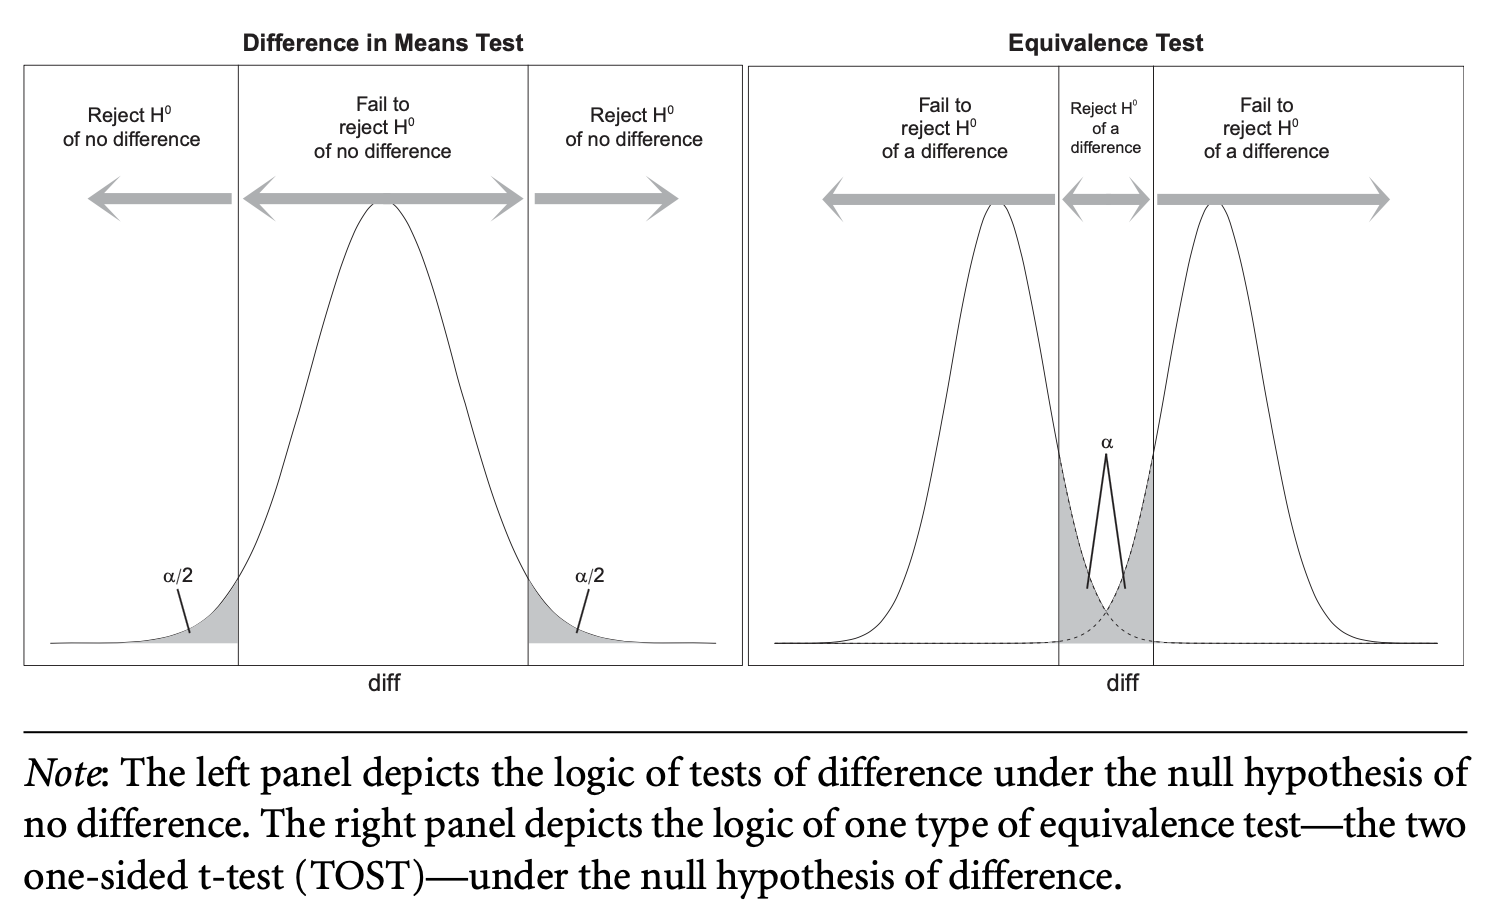
\includegraphics[trim=0 .5em 0 .5em,clip,width = 0.8\textwidth]{TOST_HH.png}\\
\end{center}
}
\end{minipage}
\end{figure}
\FloatBarrier

An alternative approach is an equivalence $F$ test, which uses the same statistic as the $F$ test:
$$F = \frac{Ntr(Ntr-m-1)}{(Ntr-1)(m+1)} \bm{\delta}_{(-m:0)}'\Sigma_{\bm{\delta}_{(-m:0)}}\bm{\delta}_{(-m:0)}$$
where $\bm{\delta}_{(-m:0)}= (ATT_{-m},ATT_{-(m-1)},\dots, ATT_{0})'$ and $\Sigma_{\bm{\delta}_{(-m:0)}}$ is the covariance matrix of $\bm{\delta}_{(-m:0)}$. The key difference lies in that we impose a reversed null hypothesis for the equivalence test:
$$H_0: \quad \bm\delta_{(-m:0)}'\Sigma_{\bm\delta_{(-m:0)}}\bm\delta_{(-m:0)} > \kappa,$$
\citet{wellek2010testing} shows that under this hypothesis, the statistic converges to a non-central $F$-distribution $F(m+1, N_{tr}-m-1, N_{tr}\kappa^2)$, where $N_{tr}\kappa^2$ is the distribution's centrality parameter. The null is considered rejected (hence, equivalence holds) when the statistic's value is smaller than the $100\alpha$th percentile of the distribution. When the absolute values of all the $ATT_{s}$ are smaller, there will be a higher chance to reject the null . Based on the discussion in \citet{wellek2010testing} and simulation results, we recommend to set $\kappa = 0.6$. 


We compare the distribution of the $F$ test with that of the equivalence test in Figure~\ref{fg:fvse} above. The solid black curve represents the distribution of the test statistic under the null of the $F$ test. The dotted black curve represents its distribution under the null of the equivalence test. We reject the null under the former if the value of the test statistic falls on the right side of the solid red line and reject the null under the latter if it falls on the left side of the dotted red line, i.e., the equivalence threshold. 

In the above case (with a chosen equivalence threshold of 0.6), the equivalence test is more lenient than the $F$ test: when the test statistic falls between the two red lines, we reject the null under the $F$ test (suggesting inequivalence), but also reject the null under the equivalence test (declaring equivalence). Therefore, the equivalence test has the same advantages as the TOST does. However, because its threshold is less intuitive and harder to interpret, we choose the TOST as the primary approach to conduct the equivalence test. 

\begin{figure}[!th]
\caption{F distribution under the Two Tests}\label{fg:fvse}
\centering
\begin{minipage}{0.85\linewidth}{
\begin{center}
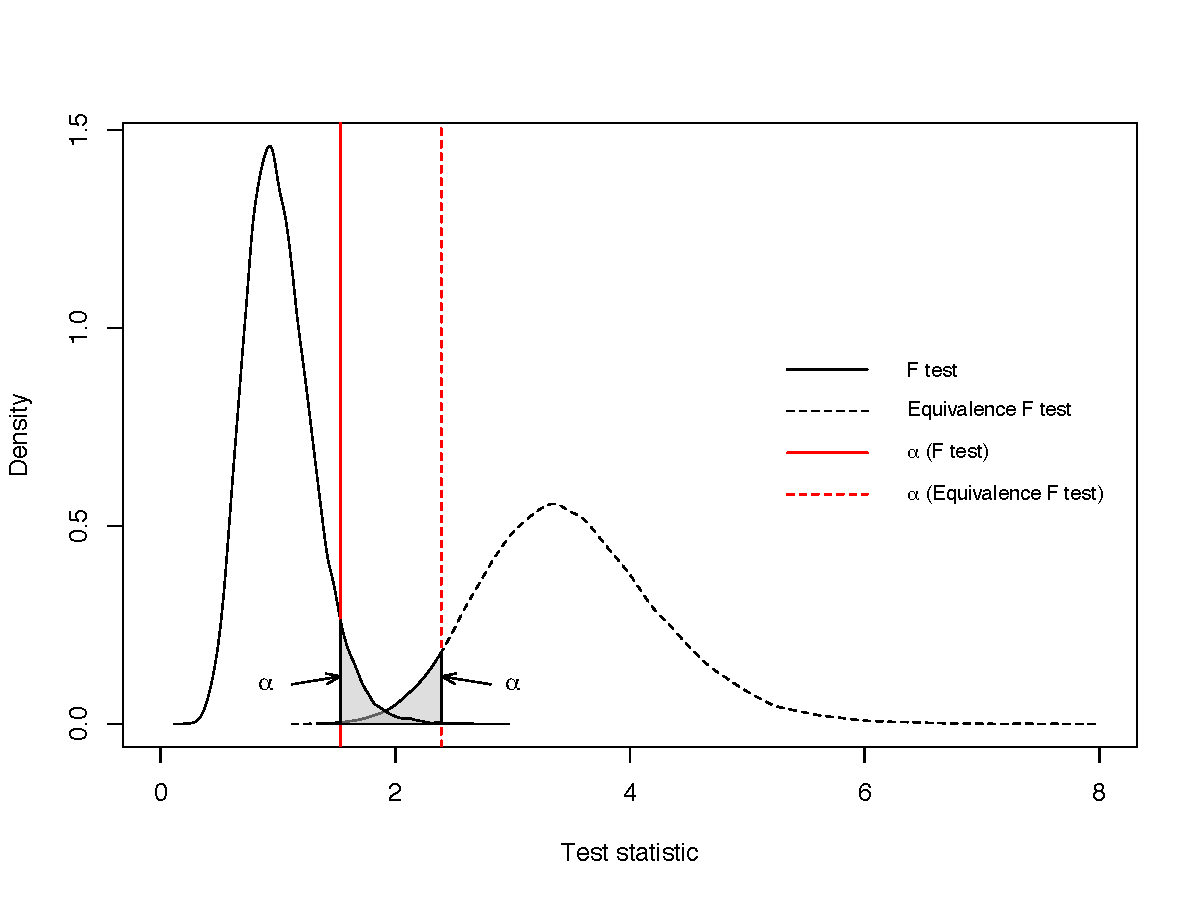
\includegraphics[trim=0 1em 0 4em,clip,width = 0.8\textwidth]{F_Distribution.pdf}\\
\end{center}
}
\footnotesize\textbf{Note:} The above figure plots the distribution of the test statistic under the null of the $F$ test and its distribution under the null of the equivalence test. The shaded areas represent the size of the two tests ($\alpha = 0.05)$. 
\end{minipage}
\end{figure}

\bigskip
\clearpage

\subsection{Discussion on the No Carryover Effects Assumption}\label{sc:no-co}

The violation of no carryover effects assumption is a violation of the stable unit treatment value assumption (SUTVA) along the temporal dimension, i.e., the potential outcome of unit $i$ in period $t$ could be affected by its own treatment status in earlier periods. Therefore, the presence of carryover effects is equivalent to temporal interference and does not imply failure of the strict exogeneity assumption. 

As we briefly discuss in the main text, violations of the no carryover effects assumption is not a concern under staggered adoption; it is a concern when the treatment switches on and off for some unit. In the latter case, the carryover effects can be seen as a result of special ``time-varying confounders.'' Hence, we can use the placebo test introduced earlier in paper to gauge whether they exist. When the average prediction error in those periods deviate from zero, we obtain a piece of evidence that the assumption is likely invalid (of course, it is also possible it is a result of some temporal shocks unrelated to carryover effects). A potential solution in this scenario is to re-code the treatment such that we label a few periods after the treatment's ending as under treatment to allow the carryover effects to fully present themselves.
\begin{figure}[!ht]
\caption{Illustrating Carryover Effects under Staggered Adoption}\label{fg:carryover}
\vspace{0.5em}
\centering
\begin{minipage}{1\linewidth}{
\begin{center}
\hspace{1em}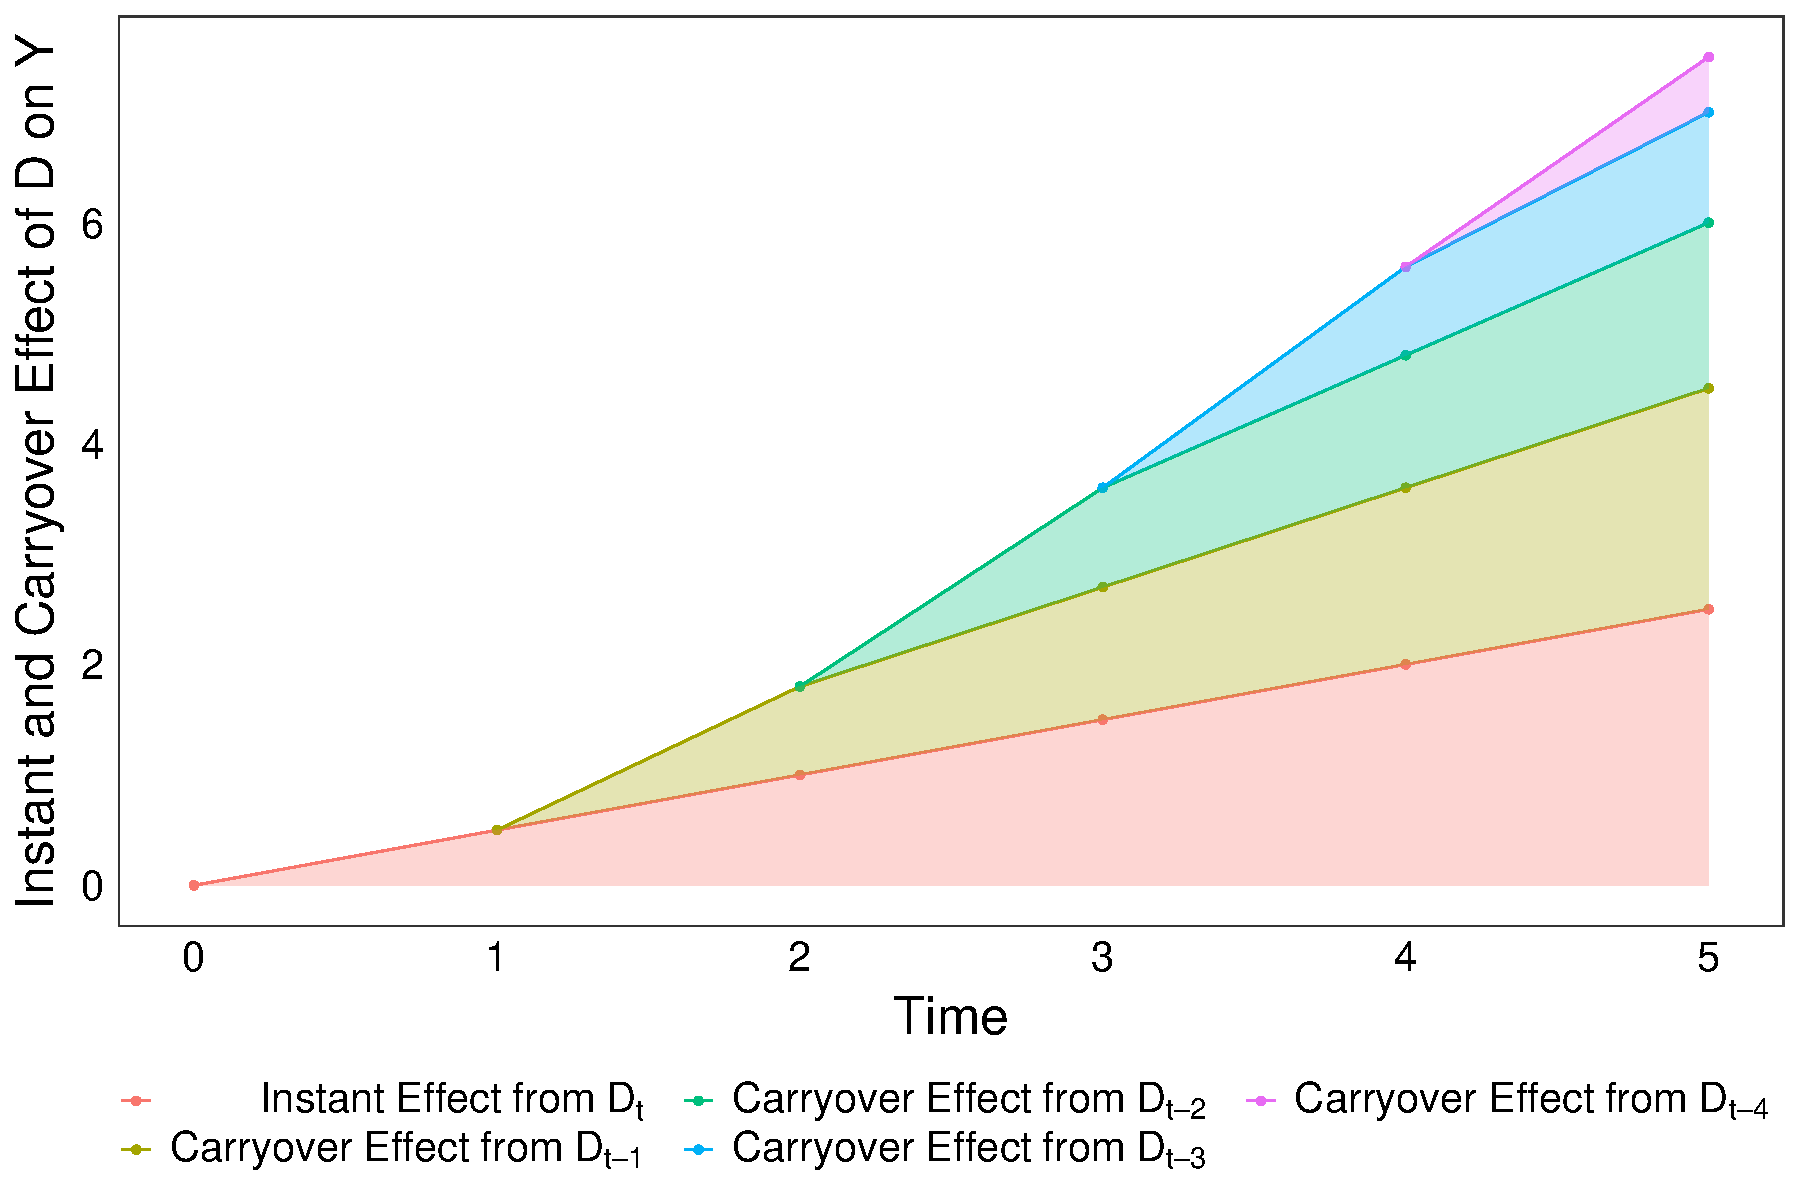
\includegraphics[width = 0.7\textwidth]{carryover.pdf}
\end{center}
\footnotesize\textbf{Note:} The above figures demonstrates a decomposition of $\delta_{it}$ in a hypothetical case under staggered adoption when carry over effects exist. The x-axis indicates the time relative the onset of the treatment.}
\end{minipage}\vspace{-0.5em}
\end{figure}

Under staggered adoption, however, we may not be concerned about the carryover effect because we can reinterpret $\delta_{it}$ as a combination of the instant effect of the current treatment (red area in Figure~\ref{fg:carryover}) and cumulative carryover effects of past treatments (other colored areas) on a treated unit $i$ relative to its potential outcome history under the never-treated condition. 


\clearpage

\subsection{Procedures for the Diagnostic Tests}

We describe the procedures for the diagnostic tests below. Figure~\ref{fg:tests}(a) and (b) illustrate how the placebo test and test for no carryover effects are performed, respectively.

\begin{figure}[!ht]
\caption{Illustrating the Diagnostic Tests}\label{fg:tests}
\centering
\begin{minipage}{0.95\linewidth}
\begin{center}
\hspace{-2em}
\subfigure[Placebo Test]{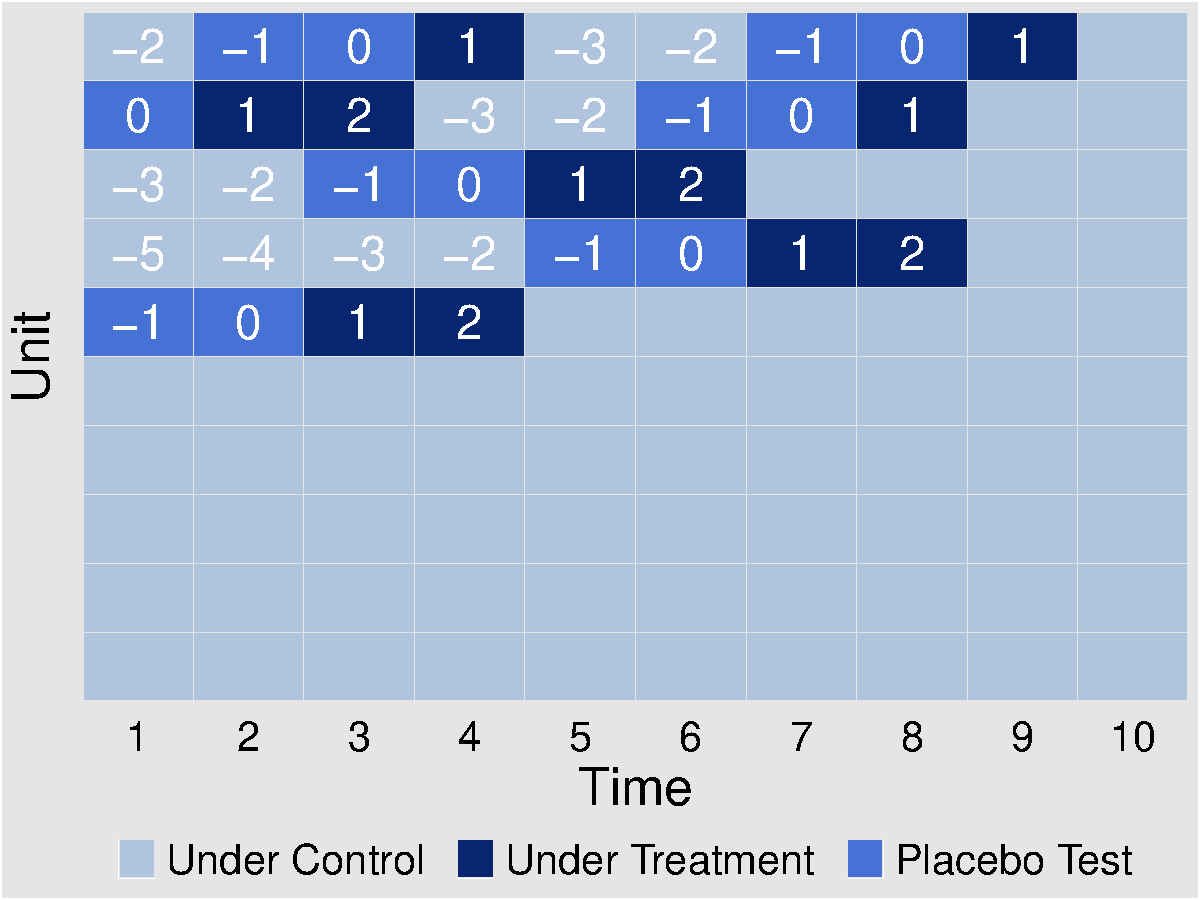
\includegraphics[width = 0.45\textwidth]{treat_placebo.pdf}}\hspace{2em}
\subfigure[Test for No Carryover Effects]{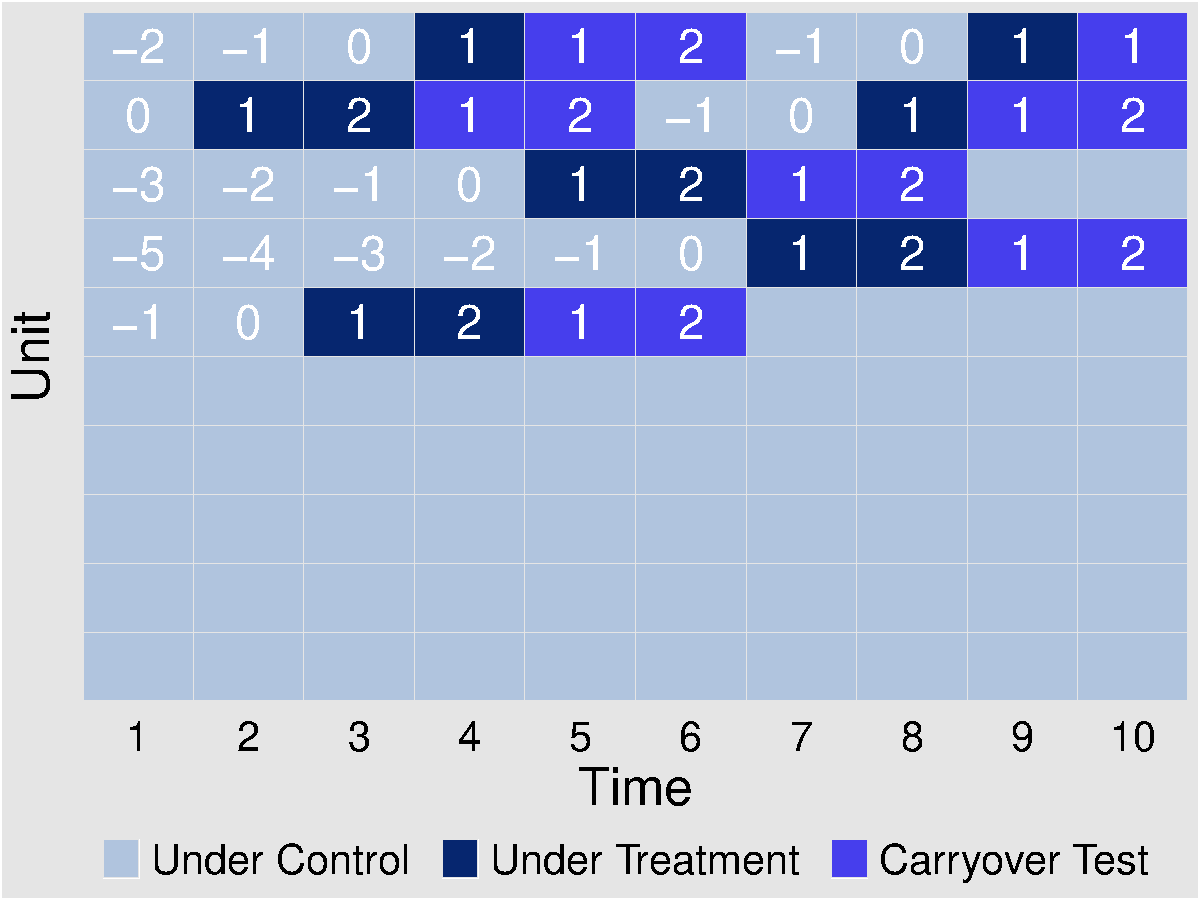
\includegraphics[width = 0.45\textwidth]{treat_carryover.pdf}}\\
\end{center}
\footnotesize\textbf{Note:} The above figures show how observations in periods relative to the onset or ending of the treatment are being used in the diagnostic tests. 
\end{minipage}
\vspace{-1em}
\end{figure}


\paragraph{Placebo test.} 
\begin{enumerate}
    \item If the equivalence approach is being used, specify a significant level $\alpha$, like $\alpha = 0.05$, the length of placebo period $l$, and two equivalence thresholds $-\theta_2$ and $\theta_1$ such that 
    $-\theta_2 < 0 < \theta_1$. In in Figure~\ref{fg:tests}(a), $l = 2$ (Periods 0 and -1).
    
    \item Regard $l$ observations immediately before the onset of the treatment for each treated unit ($C_{i} = 1$) as observations under the placebo, remove them when fitting the model, and obtain an estimate for average ``treatment effect'' in placebo periods denoted as $\widehat{ATT}^P$.
    
    \item Use bootstrap or jackknife method to obtain a 
    $(1 - \alpha)$ or $(1 - 2\alpha)$ confidence interval for $\widehat{ATT}^P$. Denote 
    $\widehat{ATT}^P_u$ the upper bound and 
    $\widehat{ATT}^P_l$ the lower bound.
    
    \item Test $\widehat{ATT}^P$ against the null hypothesis using either the DIM approach or the equivalence approach.  
\end{enumerate}

\paragraph{Test for no pretrend.} The test for no pretrend is a special case of the placebo test when $l = 1$. It conducts the placebo test repeatedly by removing the $j$'th period before the treatment starts, $j = 1, 2, \cdots$ (in Figure~\ref{fg:tests}(a), the periods marked with 0, -1, -2, -3).

\paragraph{Test for no carryover effects.} 
\begin{enumerate}
    \item If the equivalence approach is being used, specify a significant level $\alpha$, like $\alpha = 0.05$, the length of carryover effect period $l$, and two equivalence thresholds $-\theta_2$ and $\theta_1$ such that $-\theta_2 < 0 < \theta_1$. In in Figure~\ref{fg:tests}(b), $l = 2$ (Periods 1 and 2 in purple).
    
    \item Regard the first $l$ observations after the ending of 
    the treatment as periods potentially under carryover effects, remove them when fitting the model, and obtain an estimate for average treatment 
    effect in carryover effect periods denoted as $\widehat{ATT}^C$.
    
    \item Use bootstrap or jackknife method to obtain a 
    $(1 - \alpha)$ or $(1 - 2\alpha)$ confidence interval for $\widehat{ATT}^C$. Denote 
    $\widehat{ATT}^C_u$ the upper bound and 
    $\widehat{ATT}^C_l$ the lower bound.

    \item Test $\widehat{ATT}^C_u$ against the null hypothesis using either the DIM approach or the equivalence approach.  
\end{enumerate}



\paragraph{Allowing limited carryover effects.} Sometimes, as in \citet{FM2015-yy}, researchers may find evidence for limited carryover effects. Researchers can thus specify the number periods after the treatment's ending that allow carryover effects can take place. After removing those periods, researchers can then proceed to re-estimate the ATT and re-conduct the diagnostic tests. Figure~\ref{fg:tests2} illustrate the placebo test (a) and test for no carryover effects (b) when two periods after the treatment's ending (in sky blue) are removed. We apply this method in drawing Figure 10 in the main text. 

\begin{figure}[!ht]
\caption{Illustrating the Diagnostic Tests\\Allowing Limited Carryover Effects (Up to Two Periods)}\label{fg:tests2}
\centering
\begin{minipage}{0.95\linewidth}
\begin{center}
\hspace{-2em}
\subfigure[Placebo Test]{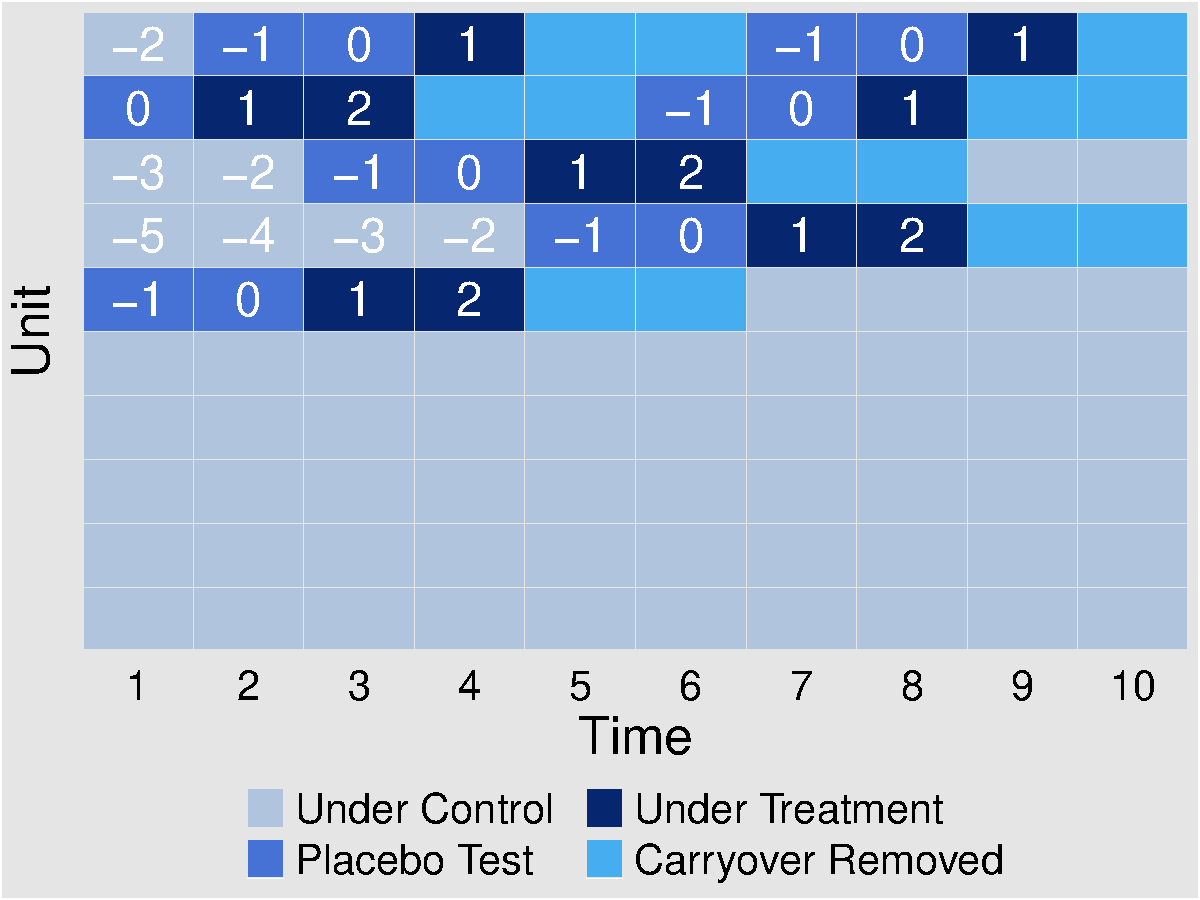
\includegraphics[width = 0.45\textwidth]{treat_crm_placebo.pdf}}\hspace{2em}
\subfigure[Test for No Carryover Effects]{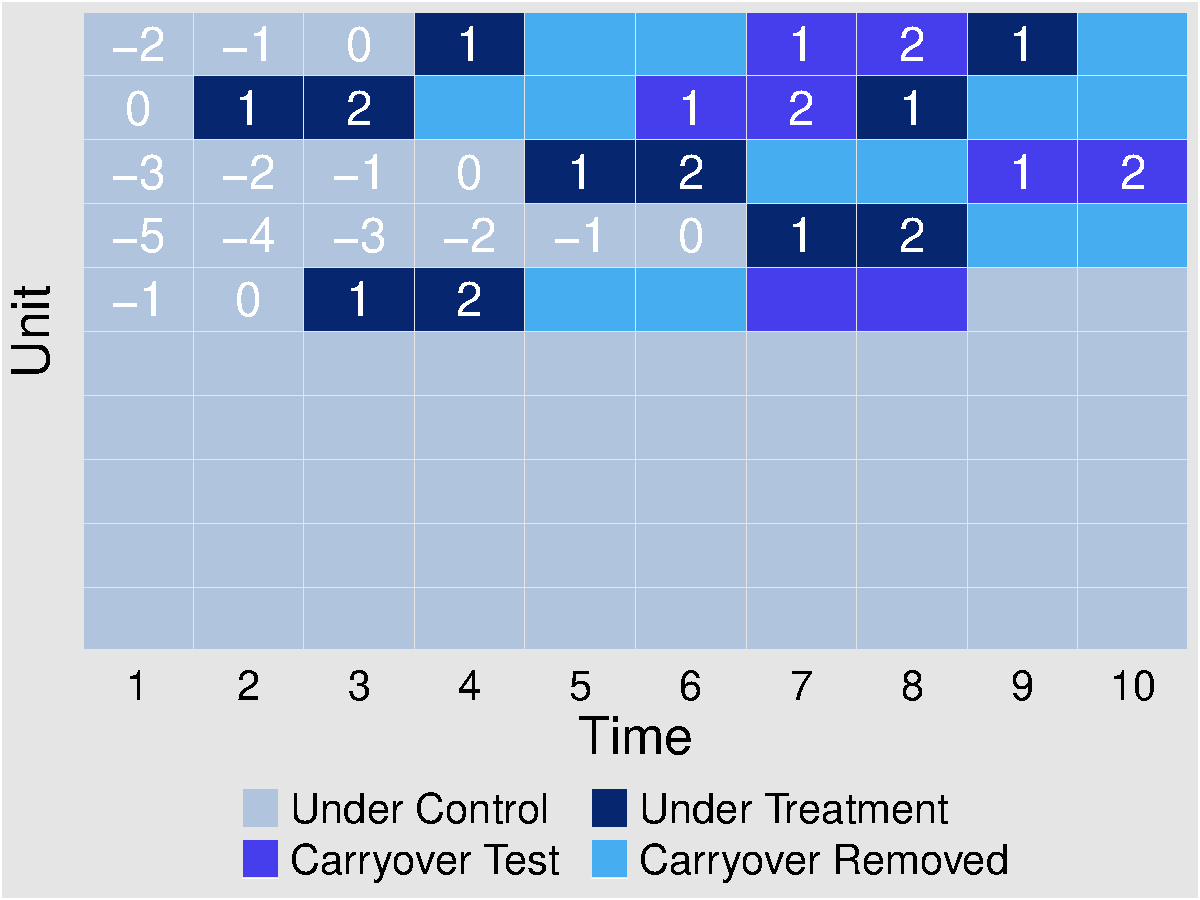
\includegraphics[width = 0.45\textwidth]{treat_crm_carryover.pdf}}\\
\end{center}
\footnotesize\textbf{Note:} The above figures show how observations in periods relative to the onset and ending of the treatment are being used in the diagnostic tests. 
\end{minipage}
\vspace{-1em}
\end{figure}

\clearpage


%%%%%%%%%%%%%%%%%%%%%%%%%%%%%%%%%%%%%%%%%%%%%%%%%%%%%%%%%%%%%%%%%%%%%%%%%%%%%%%%%%%%%%%%%%%%%%%%%%%%%%%%%%%%%%%%%%%%%%%%%%%%%%%%%%%%%%%%%%%%%%%%%%%%%%%%%%%%%%%%%%%%%%%%%%%%%%%%%%%%%%%%%%%%%%%%%%%%%%%%%%%%%%%%%%%%%%%%%%%%%%%%%%%%%%%%%%%%%%%%%%%%%%%%%%%%%%%%%%%%%%%%%%%%%%%%%%%%%%%%%%%%%%%%%%%%%%%%%%%%%%%%%%%%%%%%%%%%%%%%%%%%%%%%%%%%%%%%%%%%%%%%%%%%%%%%%%%%%%%%%%%%%%%%%%%%%%%%%%%%%%%%%%%%%%%%%%%%%%%%%%%%%%%%%%%%%%%%%%%%%%%%%%%%%%%%%%%%%%%%%%%%%%%%%%%%%%%%%%%%%%%%%%%%%%%%%%%%%%%%%%%%%%%%%%%%%%%%%%%%%%%%%%%%%%%%%%%%%%%%%%%%%%%%%%%%%%%%%%%%%%%%%%%%%%%%%%%%%%%%%%%%%%%%%%%%%%%%%%%%%%%%%%%%%%%%%%%%%%%%%%%%%%%%%%%%%%%%%%%%%%%%%%%%%%%%%%%%%%%%%%%%%%%%%%%%%%%%%%%%%%%%%%%%%%%%%%%%%%%%%%%%%%%%%%%%%%%%%%%%%%%%%%%%%%%%%%%%%%%%%%%%%%%%%%%%%%%%%%%%%%%%%%%%%%%%%%%%%%%%%%%%%%%%%%%%%%%%%%%%%%%%%%%  
%%%%%%%%%%%%%%%%%%%%%%%%%%%%%%%%%%%%%%%%%%%%%%%%%%%%%%%%%%%%%%%%%%%%%%%%%%%%%%%%%%%%%%%%%%%%%%%%%%%%%%%%%%%%%%%%%%%%%%%%%%%%%%%%%%%%%%%%%%%%%%%%%%%%%%%%%%%%%%%%%%%%%%%%%%%%%%%%%%%%%%%%%%%%%%%%%%%%%%%%%%%%%%%%%%%%%%%%%%%%%%%%%%%%%%%%%%%%%%%%%%%%%%%%%%%%%%%%%%%%%%%%%%%%%%%%%%%%%%%%%%%%%%%%%%%%%%%%%%%%%%%%%%%%%%%%%%%%%%%%%%%%%%%%%%%%%%%%%%%%%%%%%%%%%%%%%%%%%%%%%%%%%%%%%%%%%%%%%%%%%%%%%%%%%%%%%%%%%%%%%%%%%%%%%%%%%%%%%%%%%%%%%%%%%%%%%%%%%%%%%%%%%%%%%%%%%%%%%%%%%%%%%%%%%%%%%%%%%%%%%%%%%%%%%%%%%%%%%%%%%%%%%%%%%%%%%%%%%%%%%%%%%%%%%%%%%%%%%%%%%%%%%%%%%%%%%%%%%%%%%%%%%%%%%%%%%%%%%%%%%%%%%%%%%%%%%%%%%%%%%%%%%%%%%%%%%%%%%%%%%%%%%%%%%%%%%%%%%%%%%%%%%%%%%%%%%%%%%%%%%%%%%%%%%%%%%%%%%%%%%%%%%%%%%%%%%%%%%%%%%%%%%%%%%%%%%%%%%%%%%%%%%%%%%%%%%%%%%%%%%%%%%%%%%%%%%%%%%%%%%%%%%%%%%%%%%%%%%%%%%%%%%%%  
%%%%%%%%%%%%%%%%%%%%%%%%%%%%%%%%%%%%%%%%%%%%%%%%%%%%%%%%%%%%%%%%%%%%%%%%%%%%%%%%%%%%%%%%%%%%%%%%%%%%%%%%%%%%%%%%%%%%%%%%%%%%%%%%%%%%%%%%%%%%%%%%%%%%%%%%%%%%%%%%%%%%%%%%%%%%%%%%%%%%%%%%%%%%%%%%%%%%%%%%%%%%%%%%%%%%%%%%%%%%%%%%%%%%%%%%%%%%%%%%%%%%%%%%%%%%%%%%%%%%%%%%%%%%%%%%%%%%%%%%%%%%%%%%%%%%%%%%%%%%%%%%%%%%%%%%%%%%%%%%%%%%%%%%%%%%%%%%%%%%%%%%%%%%%%%%%%%%%%%%%%%%%%%%%%%%%%%%%%%%%%%%%%%%%%%%%%%%%%%%%%%%%%%%%%%%%%%%%%%%%%%%%%%%%%%%%%%%%%%%%%%%%%%%%%%%%%%%%%%%%%%%%%%%%%%%%%%%%%%%%%%%%%%%%%%%%%%%%%%%%%%%%%%%%%%%%%%%%%%%%%%%%%%%%%%%%%%%%%%%%%%%%%%%%%%%%%%%%%%%%%%%%%%%%%%%%%%%%%%%%%%%%%%%%%%%%%%%%%%%%%%%%%%%%%%%%%%%%%%%%%%%%%%%%%%%%%%%%%%%%%%%%%%%%%%%%%%%%%%%%%%%%%%%%%%%%%%%%%%%%%%%%%%%%%%%%%%%%%%%%%%%%%%%%%%%%%%%%%%%%%%%%%%%%%%%%%%%%%%%%%%%%%%%%%%%%%%%%%%%%%%%%%%%%%%%%%%%%%%%%%%%%%% 

\clearpage


\section{Proofs}

\subsection{Unbiasedness and Consistency of FEct and IFEct}

Denote the number of all observations, the number of observations with $D_{it} = 1$, and the number of observations with $D_{it} = 0$ as $n$, $n_{\mathcal{M}}$, and $n_{\mathcal{O}}$, respectively. Under FEct, our Assumptions 1, 2, and 3 lead to the following model specification:
  \begin{align}
   Y_{it} = \mathbf{X}_{it}'\beta & + \alpha_{i} + \xi_{t} +
  \varepsilon_{it},  \hspace{1mm} (i, t) \in \mathcal{O},   \label{aeq.sp}\\
  & \sum_{D_{it} = 0}\alpha_{i} =  \sum_{D_{it} = 0} \xi_t, \notag \\
 \varepsilon_{it} \perp \{D_{js}, & \mathbf{X}_{js} , \alpha_{j}, \xi_{s}\} \text{ for any } i,j \in \{1,2,\dots,N\} \text{ and } s,t \in \{1,2,\dots,T\}. \notag
   \end{align}   
The data we use to estimate these parameters constitute an unbalanced panel since we are not using observations whose $D_{it}=1$. Following \citet{wansbeek1989estimation}, we rearrange the observations so that data on $N$ units ``are ordered in $T$ consecutive sets," thus the index $t$ ``runs slowly" and $i$ ``runs quickly." Denote the number of untreated units in period $t$ as $N_t$, then $N_t \leq N$ and $\sum_{t=1}^{T} N_t = n_{\mathcal{O}}$, the number of untreated observations in the dataset. Similarly, denote the number of periods in which unit $i$ is untreated as $T_i$. Then $T_i \leq T$ and $\sum_{i=1}^{N} T_i = n_{\mathcal{O}}$.  Let $M_t$ be the $N_t \times N$ matrix where row $i$ equals to the corresponding row in the unit matrix $I_{N}$ if $i$ is observed in period $t$. Then we can rewrite Equation (\ref{aeq.sp}) in the matrix form:
\begin{equation*}
Y = \mathbf{X} \beta + \Delta (\alpha, \xi)' + \varepsilon
\end{equation*}
  where $\mathbf{X} = (\mathbf{x}_{11}, \mathbf{x}_{21}, \cdots, \mathbf{x}_{NT})'$ is a $n_{\mathcal{O}} \times K$ matrix, $\iota_n$ denotes the $n_{\mathcal{O}}$-dimension vector consisted of 1s, $\Delta = (\Delta_{1}, \Delta_{2})$,  $\Delta_{1} = \begin{pmatrix}
  \mathbf{M}_1 \\
  \mathbf{M}_2 \\
  \vdots \\
  \mathbf{M}_T
  \end{pmatrix}$, and $\Delta_{2} = \begin{pmatrix}
  \mathbf{M}_1 \iota_{N} & & &    \\
  & \mathbf{M}_2 \iota_{N} \\
  & & \ddots \\
  & & & \mathbf{M}_T \iota_{N}
  \end{pmatrix}$. \\

Under IFEct, the model specification that satisfies Assumptions 1, 2, and 3 has the following form:
   \begin{align}
 &  Y_{it} = \mathbf{X}_{it}'\beta + \mathbf{\lambda}_{i}^{'} f_{t} + \alpha_{i} + \xi_{t} + \varepsilon_{it},  \hspace{1mm} D_{it}=0, \\
 & \sum_{D_{it} = 0}\alpha_{i} = 0,  \sum_{D_{it} = 0} \xi_t = 0, \mathbf{\Lambda}' \mathbf{\Lambda} = diagnal, \mathbf{F}'\mathbf{F} / T = \mathbf{I}_r,  \notag \\
 & \varepsilon_{it} \perp \{D_{js}, \mathbf{X}_{js} , \alpha_{j}, \xi_{s}, \mathbf{\lambda}_{j}, f_{s}\} \text{ for any } i,j \in \{1,2,\dots,N\} \text{ and } s,t \in \{1,2,\dots,T\}. \notag
   \end{align}   
 in which $\mathbf{\Lambda} = \left[\lambda_1, \lambda_2, \hdots, \lambda_N \right]'$ and $\mathbf{F} = \left[f_1, f_2, \hdots, f_T \right]'$. 
  % the consistency of beta
From now on we denote the projection matrix of matrix $\mathbf{A}$ as $P_{\mathbf{A}}$  and the corresponding residual-making matrix as $Q_{\mathbf{A}}$.

Proving the ATT estimator's consistency requires some regularity conditions. First, following \citet{Bai2009} and \citet{xu2017generalized}, we assume that the error terms have weak serial dependence:

\noindent\textbf{Weak serial dependence:}\\
1. $E\left[\varepsilon_{it} \varepsilon_{is} \right] = \sigma_{i,ts}, |\sigma_{i,ts}| \leq \bar{\sigma}_i$ for all $(t,s)$ such that $\frac{1}{N}\sum_i^N \bar{\sigma}_i < M$. \\
2. For every $(t,s)$, $E\left[N^{-1/2} \sum_i^N \varepsilon_{it} \varepsilon_{is} - E\left[\varepsilon_{it} \varepsilon_{is} \right] \right]^4 \leq M$. \\
3. $\frac{1}{NT^2} \sum_{t,s,u,v}\sum_{i,j}|cov\left[\varepsilon_{it} \varepsilon_{is}, \varepsilon_{ju} \varepsilon_{jv} \right]| \leq M$ and\\
$\frac{1}{N^2T} \sum_{t,s}\sum_{i,j,k,l}|cov\left[\varepsilon_{it} \varepsilon_{jt}, \varepsilon_{ks} \varepsilon_{ls} \right]| \leq M$.\\
4. $E\left[\varepsilon_{it} \varepsilon_{js} \right] = 0$ for all $i \neq j$, $(t,s)$. \\
These assumptions imply Assumption 3 in \citet{MoonWeidner2013} that $\frac{||\varepsilon||}{NT} \rightarrow 0$ as $N, T$ go to infinity. We also need some restrictions on parameters in the models:

\noindent\textbf{Restriction on parameters:}\\
1.  For each $t$, $\frac{N_t}{N} \rightarrow p_t$ as $N \rightarrow \infty$, where $0 \leq p_t < 1$ is a constant that varies with $t$.  \\
2. All entries of the matrix $E\left[\mathbf{x_{it}}\mathbf{x_{it}}' \right]$ is bounded by $M$. \\
3. For each unit $i$, all the covariates have weak serial dependence: $\sum_{t}^{T_i}X_{it, j} \times \sum_{t}^{T_i}X_{it, k} \leq M$ for any $(k, j)$. \\
4. Define $W(\lambda)$ as $\{\frac{1}{N}tr \left(\mathbf{x}^{'}_{k_1}Q_{\lambda}\mathbf{x}_{k_2}Q_{\mathbf{F}} \right)\}_{K \times K}$ and $w(\lambda)$ as the smallest eigenvalue of $W(\lambda)$. Define $W(f)$ as $\{\frac{1}{N}tr \left(\mathbf{x}_{k_1}Q_{f}\mathbf{x}^{'}_{k_2}Q_{\mathbf{\Lambda}} \right)\}_{K \times K}$ and $w(f)$ as the smallest eigenvalue of $W(f)$. Then either $\lim_{N,T \rightarrow \infty} min_{\lambda}\text{ } w(\lambda) > 0$, or $\lim_{N,T \rightarrow \infty} min_{f}\text{ } w(f) > 0$ holds. 

The last restriction comes from \citet{MoonWeidner2013} for the consistency of the IFEct model.

\begin{lemma}
Under model specification (A1) and regularity conditions, all the following limits\footnote{All the convergences here are convergence in probability.} exist: 
$(a) \lim_{N \rightarrow \infty} \frac{\mathbf{X}'\mathbf{X}}{N}$, 
$(b) \lim_{N \rightarrow \infty} \frac{\mathbf{X}'\epsilon}{N}$, 
$(c) \lim_{N \rightarrow \infty} \frac{\mathbf{X}'\Delta_2}{N}$, 
$(d) \lim_{N \rightarrow \infty} \frac{\Delta_2'\Delta_2}{N}$, 
$(e) \lim_{N \rightarrow \infty} \frac{\Delta_1'\Delta_1}{N}$,\\ 
$(f) \lim_{N \rightarrow \infty} \frac{\mathbf{X}'\Delta_1 diag\{\frac{1}{T_i}\}\mathbf{X}\Delta_1'}{N}$, where $diag\{\frac{1}{T_i}\}$ is a diagonal matrix with $\frac{1}{T_i}$ being the ith entry on the diagonal. 
\end{lemma}
\begin{proof} We start from proving (a). When the regularities conditions are satisfied, we can apply the weak law of large numbers:
\begin{align*}
\lim_{N \rightarrow \infty} \frac{\mathbf{X}'\mathbf{X}}{N} = \lim_{N \rightarrow \infty} \frac{\sum_{i}^{N} \sum_{t}^{T_i} \mathbf{x}_{it}\mathbf{x}_{it}^{'}}{N} =  \frac{\sum_{i}^{N} \sum_{t}^{T_i}
E\left[\mathbf{x}_{it}\mathbf{x}_{it}^{'}\right]}{N} = \bar{T}_i  E\left[\mathbf{x}_{it}\mathbf{x}_{it}' \right]
\end{align*}
which is bounded by $\bar{T}_i M$.
Similarly,
\begin{align*}
\lim_{N \rightarrow \infty} \frac{\mathbf{X}'\mathbf{\varepsilon}}{N} = \bar{T}_i  E\left[\mathbf{x}_{i,t}\mathbf{\varepsilon_{i,t}}' \right] = \mathbf{0}_{NT \times 1}
\end{align*}
For (c), we know that
\begin{align*}
\lim_{N \rightarrow \infty} \frac{\mathbf{X}'\Delta_2}{N} & = \lim_{N \rightarrow \infty} \frac{\sum_{i}^{N} \sum_{t}^{T_i} \mathbf{x}_{it}\Delta_{2, it}^{'}}{N}   =  \frac{\sum_{i}^{N} E\left[\sum_{t}^{T_i} \mathbf{x}_{it}\Delta_{2, it}^{'}\right]}{N} = \frac{\sum_{i}^{N} E\left[\mathbf{A}_i \right]}{N}
\end{align*}
where $\mathbf{A}_i$ is a $K \times T$ matrix, and the $t$th column of $\mathbf{A}_i$ equals to $\mathbf{0}_{K \times 1}$ when $D_{it} = 1$ and equals to $\mathbf{x}_{it}$ when $D_{it} = 0$. Clearly the limit exists under regularity conditions.

(d) and (e) are obvious.
For (f), 
\begin{align*}
& \lim_{N \rightarrow \infty} \frac{\mathbf{X}'\Delta_1 diag\{\frac{1}{T_i}\}  \mathbf{X}\Delta_1'}{N} \\
= & \lim_{N \rightarrow \infty} \frac{\sum_i^N \{\sum_{t}^{T_i}X_{it, j} \times \sum_{t}^{T_i}X_{it, k} / T_i\}_{K\times K}}{N} \\
= & \frac{\sum_i^N E\left[\frac{\mathbf{B}_i  }{T_i}\right]}{N}
\end{align*}
where $\mathbf{B}_i$ is a $K \times K$ matrix and the $(j, k)$th entry of $\mathbf{B}_i$ is $\sum_{t}^{T_i}X_{it, j} \times \sum_{t}^{T_i}X_{it, k}$. It is bounded by $\frac{M}{T_i}$.
(g) can be similarly proven.
\end{proof}

\begin{lemma}
Under model specification (A1) and regularity conditions, a. estimates of $\beta$, $\alpha_{i}$, and $\xi_{t}$ from equations (1) to (3), i.e. $\hat{\beta}$, $\hat{\alpha}_{i}$, and $\hat{\xi}_{t}$, are unbiased, and b. $\hat{\beta}$ and $\hat{\xi}_{t}$ are consistent as $N \rightarrow \infty$.
\end{lemma}

\begin{proof}
\noindent  As shown in \citet{wansbeek1989estimation}, $\beta$ under model specification (A1) can still be estimated using the within estimator. Multiplying both sides of demeaned equation (4) with $Q_{[\Delta]}$, we have $Q_{[\Delta]} Y = Q_{[\Delta]} \mathbf{X} \beta + Q_{[\Delta]} \varepsilon$, then it is easy to show that:
\begin{align*}
\hat{\beta} & = (\mathbf{X}' Q_{[\Delta]} \mathbf{X})^{-1}\mathbf{X}' Q_{[\Delta]} Y = (\mathbf{X}' Q_{[\Delta]} \mathbf{X})^{-1}\mathbf{X}' Q_{[\Delta]} [\mathbf{X} \beta + \Delta (\alpha, \xi)' + \varepsilon] \\
 & = \beta + (\mathbf{X}' Q_{[\Delta]} \mathbf{X})^{-1}X' Q_{[\Delta]}  \varepsilon
\end{align*}   
   Hence, $E[\hat{\beta}] = \beta + E[(\mathbf{X}' Q_{[\Delta]} \mathbf{X})^{-1}\mathbf{X}' Q_{[\Delta]}  \varepsilon] = \beta$, and $E[\hat{\mu}] = E[\bar{Y} - \bar{X} \hat{\beta}] = \bar{Y} - \bar{X}\beta = \mu$. \\ \\
   Similarly, 
   \begin{align*}
   Q_{[\mathbf{X}]}Y = Q_{[\mathbf{X}]}\Delta (\alpha, \xi)' + Q_{[\mathbf{X}]} \varepsilon
   \end{align*}
  The level of fixed effects, $(\alpha, \xi)'$, can also be estimated using ordinary least squares under the two constrains (2) and (3), which is equivalent to the following constrained minimization problem:
\begin{align*}
& Min_{\gamma} \quad (Q_{[\mathbf{X}]}Y - Q_{[\mathbf{X}]}\Delta \gamma)'(Q_{[\mathbf{X}]}Y - Q_{[\mathbf{X}]}\Delta \gamma) \\
& with \quad \Pi \gamma = 0
\end{align*}
where $\gamma = (\alpha, \xi)'$, and $\Pi_{1 \times (N + T)} = \begin{pmatrix}
  T_1, T_2, \hdots, T_N, -N_1, -N_2, \hdots, -N_T 
\end{pmatrix}$. \\
The solution to the minimization problem is given by the following equation: 
\begin{align*}
\Phi \begin{pmatrix}
  \hat{\gamma} \\
  \hat{\lambda}
\end{pmatrix} = 
\begin{pmatrix}
  \Delta' Q_{[\mathbf{X}]} \Delta, & \Pi' \\
  \Pi, & 0
\end{pmatrix} \begin{pmatrix}
  \hat{\gamma} \\
  \hat{\lambda}
\end{pmatrix} = \begin{pmatrix}
  \Delta' Q_{[\mathbf{X}]} Y \\
  0
\end{pmatrix}
\end{align*}
where $\lambda$ represents the corresponding Lagrangian multipliers. Finally, $\hat{\gamma} = (\hat{\alpha}, \hat{\xi})' = \Phi^{-1}_{11} \Delta' Q_{[\mathbf{X}]} Y$. Here $\Phi^{-1}_{11}$ is the upper-left block of $\Phi^{-1}$. 
For unbiasedness of these estimates, notice that
\begin{align*}
E(\hat{\alpha}, \hat{\xi})' & = E[\Phi^{-1}_{11} \Delta' Q_{[\mathbf{X}]} Y] \\
& = E[\Phi^{-1}_{11} \Delta' Q_{[\mathbf{X}]} \Delta (\alpha, \xi)'] \\
& = E[(I - \Phi^{-1}_{12}\Pi)(\alpha, \xi)'] \\
& = (\alpha, \xi)'.
\end{align*}
\noindent The second equality uses the fact that $Q_{[\mathbf{X}]}\mathbf{X} = 0$. The third equality builts upon the definition of $\Phi^{-1}_{11}$ and $\Phi^{-1}_{12}$: $\Phi^{-1}_{11} \Delta' Q_{[\mathbf{X}]}\Delta + \Phi^{-1}_{12}\Pi = I$. The last equality exploits the constraint $\Pi (\alpha, \xi)' = 0$.

Now, for $\hat{\beta}$ and $\hat{\xi}$, it is easy to show that:
\begin{align*}
\lim_{N \rightarrow \infty} \begin{pmatrix}
\hat{\beta} \\
\hat{\xi}
\end{pmatrix}  = & \begin{pmatrix}
\beta \\
\xi
\end{pmatrix}  + \lim_{N \rightarrow \infty}\left[\begin{pmatrix}
\mathbf{X}'\\
\Delta_{2}^{'}
\end{pmatrix} Q_{[\Delta_1]} (\mathbf{X}, \Delta_{2})\right]^{-1}\left[\begin{pmatrix}
\mathbf{X}'\\
\Delta_{2}^{'}
\end{pmatrix} Q_{[\Delta_1]} \varepsilon \right] \\
& \begin{pmatrix}
\beta \\
\xi
\end{pmatrix}  + \lim_{N \rightarrow \infty}\left[\begin{pmatrix}
\mathbf{X}'\\
\Delta_{2}^{'}
\end{pmatrix} Q_{[\Delta_1]} (\mathbf{X}, \Delta_{2}) / N \right]^{-1}\left[\begin{pmatrix}
\mathbf{X}'\\
\Delta_{2}^{'}
\end{pmatrix} Q_{[\Delta_1]} \varepsilon / N \right] 
\end{align*}
And,
\begin{align*}
\begin{pmatrix}
\mathbf{X}'\\
\Delta_{2}^{'}
\end{pmatrix} & Q_{[\Delta_1]} (\mathbf{X}, \Delta_{2}) = \begin{pmatrix}
\mathbf{X}'\mathbf{X} & \mathbf{X}'\Delta_{2} \\
\Delta_{2}^{'}\mathbf{X} & \Delta_{2}^{'}\Delta_{2}
\end{pmatrix} - 
\begin{pmatrix}
\mathbf{X}'\Delta_{1} \\
\Delta_{2}^{'}\Delta_{1}
\end{pmatrix} \left(\Delta_{1}^{'}\Delta_{1}\right)^{-1} (\mathbf{X}\Delta_{1}^{'}, \Delta_{2}\Delta_{1}^{'}) \\
= & \begin{pmatrix}
\mathbf{X}'\mathbf{X} & \mathbf{X}'\Delta_{2} \\
\Delta_{2}^{'}\mathbf{X} & \Delta_{2}^{'}\Delta_{2}
\end{pmatrix} - 
\begin{pmatrix}
\mathbf{X}'\Delta_{1} \\
\Delta_{2}^{'}\Delta_{1}
\end{pmatrix} diag\{\frac{1}{T_i}\} (\mathbf{X}\Delta_{1}^{'}, \Delta_{2}\Delta_{1}^{'})
\end{align*}
Using Lemma 1, we know that as $N \rightarrow \infty$, each term in the expression above will converge in probability to a fixed matrix. Using Slutsky's theorem,  $\left[\begin{pmatrix}
\mathbf{X}'\\
\Delta_{2}^{'}
\end{pmatrix} Q_{[\Delta_1]} (\mathbf{X}, \Delta_{2}) / N\right]^{-1}$ also converges to a fixed matrix. Similarly, we can show that $\left[\begin{pmatrix}
\mathbf{X}'\\
\Delta_{2}^{'}
\end{pmatrix} Q_{[\Delta_1]} \varepsilon / N \right]$ converges to $\mathbf{0}_{N \times 1}$ as $N \rightarrow \infty$, which leads to the consistency result.

On the contrary, $\hat{\alpha}_i$ is inconsistent when only $N \rightarrow \infty$ as the number of parameters changes accordingly.
\end{proof}

\begin{lemma}
Under model specification (A2) and regularity conditions, a. estimates of $\beta$, $\alpha_{i}$, $\xi_{t}$, $\lambda_{i}$, and $f_{t}$ from equations (5) to (9), i.e. $\hat{\beta}$, $\hat{\alpha}_{i}$, $\hat{\xi}_{t}$, $\hat{\lambda}_{i}$, and $\hat{f}_{t}$ are a. unbiased, and b. consistent as $N, T  \rightarrow \infty$.
\end{lemma}

\begin{proof}
\citet{MoonWeidner2013} show that all the coefficients of an IFE model can be estimated via a quasi maximum likelihood estimator and the estimates are unbiased as well as consistent when both $N$ and $T$ increase to infinity. We also know that estimates obtained from the EM algorithm converge to the quasi-MLE solution since it is the unique extrema. Hence the lemma holds due to properties of QMLE.
\end{proof}

\begin{proposition}[Unbiasedness and Consistency of FEct]: Under model specification (A1), as well as regularity conditions,
\begin{center}
    $\E[\widehat{ATT}_{s}] = ATT_{s}$; $\E[\widehat{ATT}] = ATT$;\\
    $\widehat{ATT}_{s} - ATT_{s} \overset{p}{\to} 0$; and $\widehat{ATT} - ATT \overset{p}{\to} 0$ as $N\to\infty$.
\end{center}\vspace{-1ex}
\end{proposition}



\begin{proof}
We only show the unbiasedness and consistency of $\widehat{ATT}_{s}$. For $\widehat{ATT}$, the proof is similar and omitted.
  \begin{align*}
    \widehat{ATT_{s}} & = \frac{1}{|\mathcal{S}|}
                        \sum_{(i,t) \in \mathcal{S}} \left( Y_{it} - \mathbf{X}_{it}'\hat\beta
                        - \hat\alpha_{i} - \hat\xi_{t} \right)\\
                      & = \frac{1}{|\mathcal{S}|}
                        \sum_{(i,t) \in \mathcal{S}} \left\lbrace
                        \mathbf{X}_{it}'(\beta-\hat{\beta}) +
                        (\alpha_{i} -\hat\alpha_{i})
                        + (\xi_{t} - \hat\xi_{t}) + \delta_{it} \right\rbrace  
  \end{align*}
  Using lemma 1, we know that
  \begin{align*}
   \E[\widehat{ATT_{s}}]  &= \frac{1}{|\mathcal{S}|}
                        \sum_{(i,t) \in \mathcal{S}} \left\lbrace
                        E[\mathbf{X}_{it}'(\beta-\hat{\beta})] +
                        E[\alpha_{i} -\hat\alpha_{i}]
                        + E[\xi_{t} - \hat\xi_{t}] + \delta_{it} \right\rbrace \\
                        & = \frac{1}{|\mathcal{S}|}
                        \sum_{(i,t) \in \mathcal{S}} 
                        \delta_{it} \\
                        & = ATT_{s}
  \end{align*}
Therefore, unbiasedness holds. For consistency, we know from the proof of lemma 2 that:
  \begin{align*}
 \lim_{N \rightarrow \infty}   \widehat{ATT_{s}} & =  \lim_{N \rightarrow \infty}\frac{1}{|\mathcal{S}|}
                        \sum_{(i,t) \in \mathcal{S}} \left( Y_{it} - \mathbf{X}_{it}'\hat\beta
                         - \hat\alpha_{i} - \hat\xi_{t} \right) \\
                      & = \lim_{N \rightarrow \infty} \frac{1}{|\mathcal{S}|}
                        \sum_{(i,t) \in \mathcal{S}}  \left(\delta_{it} + \alpha_{i} - \hat\alpha_{i}\right) + \bar{X}_{it}'(\beta - \hat\beta)  + (\xi_{t} - \hat\xi_{t})
  \end{align*}
Lemma 2 indicates that  as $N \rightarrow \infty$, $\hat\beta$ and $\hat\xi_{t}$ converge to $\beta$, and $\xi_t$, respectively. The only thing to be shown is $\lim_{N \rightarrow \infty} \frac{1}{\sum_{i} D_{it}}
                        \sum_{i,D_{it}=1}  \left(\alpha_{i} - \hat\alpha_{i}\right) = 0$. This is true since $E\left[\alpha_{i} - \hat\alpha_{i}\right] = 0$ and $\mathrm{Var}\left[\alpha_{i} - \hat\alpha_{i}\right]$ is bounded by the regularity conditions. Therefore $\lim_{N \rightarrow \infty}   (\widehat{ATT_{s}} - \frac{1}{|\mathcal{S}|}
                        \sum_{(i,t) \in \mathcal{S}}  \delta_{it}) = \lim_{N \rightarrow \infty}   (\widehat{ATT_{s}} - ATT_s) = 0$, consistency holds.
\end{proof}


\begin{proposition}[Unbiasedness and Consistency of IFEct]: Under model specification (A2), as well as regularity conditions,
 \begin{align*}
     \E[\widehat{ATT}_{s}] = ATT_{s} &\text{ and } \E[\widehat{ATT}] = ATT;\\
    \widehat{ATT}_{s} \overset{p}{\to}  ATT_{s} &\text{ and } 
    \widehat{ATT} \overset{p}{\to}  ATT \text{ as } N, T \to\infty.
 \end{align*}
\end{proposition}

\begin{proof} From lemma 3, we know that estimates for $\beta$, $\alpha_{i}$, $\xi_{t}$, $\lambda_{i}$, and $f_{t}$  are unbiased and consistent as $N, T  \rightarrow \infty$. Hence, $\widehat{ATT_{t}}$ and $\widehat{ATT}$ are also unbiased and consistent, following the same logic in the proof of Proposition 1.
\end{proof}

\subsection{FEct as a Weighting Estimator}


\begin{proposition}[FEct as a weighting estimator]: Under model specification (A1), and when there is no covariate,
  \begin{center}
    $\widehat{ATT}_{s} = \frac{1}{|\mathcal{S}|}
                        \sum_{(i,t) \in \mathcal{S}} [Y_{it} - \mathbf{W}^{(it)'} \mathbf{Y}_{\mathcal{O}}]$,
  \end{center} 
  where $\mathbf{W}^{(it)'} = \left(\dots, W_{js}^{(it)}, \dots\right)_{(j,s) \in \mathcal{O}}$ is a vector of weights that satisfy
  \begin{align*}
  \sum_{(s: (i, s)\in\mathcal{O})}W_{is}^{(it)} = 1, \sum_{(j: (j, t)\in\mathcal{O})}W_{jt}^{(it)} = 1, \sum_{(j: s \neq t, (j, s)\in\mathcal{O})}W_{js}^{(it)} = \sum_{(s: (j \neq i, (j, s)\in\mathcal{O})}W_{js}^{(it)} = 0.
  \end{align*}
\end{proposition}

\begin{proof} When there is no covariate,
\begin{align*}
\hat\alpha_{i} + \hat\xi_{t} & = \nu_{it}' \begin{pmatrix}
  \hat{\alpha} \\
  \hat{\xi}
\end{pmatrix} = \nu_{it}' \Phi^{-1}_{11} \Delta' \mathbf{Y}_{\mathcal{O}} = \mathbf{W}^{(it)'} \mathbf{Y}_{\mathcal{O}},
\end{align*}
where $\mathbf{W}^{(it)'}  = \nu_{it}' \Phi^{-1}_{11} \Delta' = \left(\dots, W_{js}^{(it)}, \dots\right)_{(j,s) \in \mathcal{O}}$.
Therefore,
\begin{align*}
    \widehat{ATT_{s}} & = \frac{1}{|\mathcal{S}|}
                        \sum_{(i,t) \in \mathcal{S}} \left( Y_{it} - \hat       
                       \alpha_{i} - \hat\xi_{t} \right) \\
                      & = \frac{1}{|\mathcal{S}|}
                        \sum_{(i,t) \in \mathcal{S}} \left( Y_{it} - \nu_{it}' \Phi^{-1}_{11} \Delta' \mathbf{Y}_{\mathcal{O}} \right) \\
                        & = \frac{1}{|\mathcal{S}|}
                        \sum_{(i,t) \in \mathcal{S}} (Y_{it} -  \mathbf{W}^{(it)'} \mathbf{Y}_{\mathcal{O}}).
  \end{align*}
Note that 
\begin{align*}
\hat\alpha_{i} + \hat\xi_{t} & = \mathbf{W}^{(it)'} \hat{\mathbf{Y}}_{D_{it} = 0} =\mathbf{W}^{(it)'} \begin{pmatrix}
 \vdots \\
  \hat{\alpha}_j + \hat{\xi}_s \\
  \vdots
\end{pmatrix}_{(j,s) \in \mathcal{S}}.
\end{align*}
Note that under the constraints, the fixed effects are independent to each other. Hence, for the equation to hold, we must have $\sum_{(s: (i, s)\in\mathcal{O})}W_{is}^{(it)} = 1$,  $\sum_{(j: (j, t)\in\mathcal{O})}W_{jt}^{(it)} = 1$, $\sum_{(j: s \neq t, (j, s)\in\mathcal{O})}W_{js}^{(it)} = \sum_{(s: (j \neq i, (j, s)\in\mathcal{O})}W_{js}^{(it)} = 0$, as on the left-hand side there are only $\hat\alpha_{i}$ and $\hat\xi_{t}$. We can see that the weight for each untreated observation $(j, s)$ is larger if there are fewer untreated observations in unit $j$ or period $s$. 
\end{proof} \\

We now use a simple example to compare weights under the FEct estimator and those under the classic FE estimator. Consider a dataset with 3 units and 4 periods and the treatment status is as follows: 

\begin{table}[!th]
\centering
\caption{Treatment Status}\label{atb:assign}
\setlength{\extrarowheight}{2pt}
\begin{tabular}{cc|cccc|c|}
  & \multicolumn{1}{c}{} & \multicolumn{5}{c}{Periods} \\
  & \multicolumn{1}{c}{} & \multicolumn{1}{c}{$1$}  & \multicolumn{1}{c}{$2$}  & \multicolumn{1}{c}{$3$} & \multicolumn{1}{c}{$4$}  & \multicolumn{1}{c}{$\bar{D}_{i.}$} \\\cline{3-7}
            & $1$ & $0$ & $0$ & $0$ & $0$ & $0$ \\ 
Units  & $2$ & $0$ & $0$ & $0$ & $1$ & $1/4$ \\\
            & $3$ & $0$ & $1$ & $1$  & $1$ & $3/4$ \\\cline{3-7}
            & $\bar{D}_{.t}$ & $0$ & $1/3$ & $1/3$  & $2/3$ & $5/6$\\\cline{3-7}
\end{tabular}
\end{table}
where $\bar{D}_{i.}$ is the average treatment status of unit $i$ and $\bar{D}_{.t}$ is the average treatment status of period $t$. We have 4 treated observations, $(2,4)$, $(3,2)$, $(3,3)$, and $(3,4)$, and 12 untreated ones. According to \citealt{de_Chaisemartin2018-iw}, the FE estimator, $\widehat{\delta}_{FE}$, equals to $\frac{1}{2}\widehat{\delta}_{24} + \frac{3}{10}\widehat{\delta}_{32} + \frac{3}{10}\widehat{\delta}_{33} - \frac{1}{10}\widehat{\delta}_{34}$, where each $w_{it} = \frac{\epsilon_{it}}{\sum_{it: (i, t) \in \mathcal{M}} \epsilon_{it}}$ and $\epsilon_{it} = D_{it} - \bar{D}_{i.} - \bar{D}_{.t} + \bar{D}$. The last estimate contributes negatively to the ATT estimate. Meanwhile, the FEct estimator, $\widehat{\delta}_{FEct}$, equals to $\frac{1}{4}\widehat{\delta}_{24} + \frac{1}{4}\widehat{\delta}_{32} + \frac{1}{4}\widehat{\delta}_{33} + \frac{1}{4}\widehat{\delta}_{34}$. All the four weights are equal and positive. Under both FE and FEct, $\widehat{\delta}_{it} = \mathbf{W}^{(it)'} \mathbf{Y}_{\mathcal{O}}$, where the weights satisfy constraints in Proposition 3 (and conditions 2 and 3 in \citealt{arkhangelsky2021double}) although they specific values may vary across the two estimators.

%%%%%%%%%%%%%%%%%%%%%%%%%%%%%%%%%%%%%%%%%%%%%%%%%%%%%%%%%%%%%%%%%%%%%%%%%%%%%%%%%%%%%%%%%%%%%%%%%%%%%%%%%%%%%%%%%%%%%%%%%%%%%%%%%%%%%%%%%%%%%%%%%%%%%%%%%%%%%%%%%%%%%%%%%%%%%%%%%%%%%%%%%%%%%%%%%%%%%%%%%%%%%%%%%%%%%%%%%%%%%%%%%%%%%%%%%%%%%%%%%%%%%%%%%%%%%%%%%%%%%%%%%%%%%%%%%%%%%%%%%%%%%%%%%%%%%%%%%%%%%%%%%%%%%%%%%%%%%%%%%%%%%%%%%%%%%%%%%%%%%%%%%%%%%%%%%%%%%%%%%%%%%%%%%%%%%%%%%%%%%%%%%%%%%%%%%%%%%%%%%%%%%%%%%%%%%%%%%%%%%%%%%%%%%%%%%%%%%%%%%%%%%%%%%%%%%%%%%%%%%%%%%%%%%%%%%%%%%%%%%%%%%%%%%%%%%%%%%%%%%%%%%%%%%%%%%%%%%%%%%%%%%%%%%%%%%%%%%%%%%%%%%%%%%%%%%%%%%%%%%%%%%%%%%%%%%%%%%%%%%%%%%%%%%%%%%%%%%%%%%%%%%%%%%%%%%%%%%%%%%%%%%%%%%%%%%%%%%%%%%%%%%%%%%%%%%%%%%%%%%%%%%%%%%%%%%%%%%%%%%%%%%%%%%%%%%%%%%%%%%%%%%%%%%%%%%%%%%%%%%%%%%%%%%%%%%%%%%%%%%%%%%%%%%%%%%%%%%%%%%%%%%%%%%%%%%%%%%%%%%%%%%%%  
%%%%%%%%%%%%%%%%%%%%%%%%%%%%%%%%%%%%%%%%%%%%%%%%%%%%%%%%%%%%%%%%%%%%%%%%%%%%%%%%%%%%%%%%%%%%%%%%%%%%%%%%%%%%%%%%%%%%%%%%%%%%%%%%%%%%%%%%%%%%%%%%%%%%%%%%%%%%%%%%%%%%%%%%%%%%%%%%%%%%%%%%%%%%%%%%%%%%%%%%%%%%%%%%%%%%%%%%%%%%%%%%%%%%%%%%%%%%%%%%%%%%%%%%%%%%%%%%%%%%%%%%%%%%%%%%%%%%%%%%%%%%%%%%%%%%%%%%%%%%%%%%%%%%%%%%%%%%%%%%%%%%%%%%%%%%%%%%%%%%%%%%%%%%%%%%%%%%%%%%%%%%%%%%%%%%%%%%%%%%%%%%%%%%%%%%%%%%%%%%%%%%%%%%%%%%%%%%%%%%%%%%%%%%%%%%%%%%%%%%%%%%%%%%%%%%%%%%%%%%%%%%%%%%%%%%%%%%%%%%%%%%%%%%%%%%%%%%%%%%%%%%%%%%%%%%%%%%%%%%%%%%%%%%%%%%%%%%%%%%%%%%%%%%%%%%%%%%%%%%%%%%%%%%%%%%%%%%%%%%%%%%%%%%%%%%%%%%%%%%%%%%%%%%%%%%%%%%%%%%%%%%%%%%%%%%%%%%%%%%%%%%%%%%%%%%%%%%%%%%%%%%%%%%%%%%%%%%%%%%%%%%%%%%%%%%%%%%%%%%%%%%%%%%%%%%%%%%%%%%%%%%%%%%%%%%%%%%%%%%%%%%%%%%%%%%%%%%%%%%%%%%%%%%%%%%%%%%%%%%%%%%%%%  
%%%%%%%%%%%%%%%%%%%%%%%%%%%%%%%%%%%%%%%%%%%%%%%%%%%%%%%%%%%%%%%%%%%%%%%%%%%%%%%%%%%%%%%%%%%%%%%%%%%%%%%%%%%%%%%%%%%%%%%%%%%%%%%%%%%%%%%%%%%%%%%%%%%%%%%%%%%%%%%%%%%%%%%%%%%%%%%%%%%%%%%%%%%%%%%%%%%%%%%%%%%%%%%%%%%%%%%%%%%%%%%%%%%%%%%%%%%%%%%%%%%%%%%%%%%%%%%%%%%%%%%%%%%%%%%%%%%%%%%%%%%%%%%%%%%%%%%%%%%%%%%%%%%%%%%%%%%%%%%%%%%%%%%%%%%%%%%%%%%%%%%%%%%%%%%%%%%%%%%%%%%%%%%%%%%%%%%%%%%%%%%%%%%%%%%%%%%%%%%%%%%%%%%%%%%%%%%%%%%%%%%%%%%%%%%%%%%%%%%%%%%%%%%%%%%%%%%%%%%%%%%%%%%%%%%%%%%%%%%%%%%%%%%%%%%%%%%%%%%%%%%%%%%%%%%%%%%%%%%%%%%%%%%%%%%%%%%%%%%%%%%%%%%%%%%%%%%%%%%%%%%%%%%%%%%%%%%%%%%%%%%%%%%%%%%%%%%%%%%%%%%%%%%%%%%%%%%%%%%%%%%%%%%%%%%%%%%%%%%%%%%%%%%%%%%%%%%%%%%%%%%%%%%%%%%%%%%%%%%%%%%%%%%%%%%%%%%%%%%%%%%%%%%%%%%%%%%%%%%%%%%%%%%%%%%%%%%%%%%%%%%%%%%%%%%%%%%%%%%%%%%%%%%%%%%%%%%%%%%%%%%%%%%

%\section{Additional Information on Monte Carlo Results}
\clearpage
\section{Inferential Methods}

We rely on nonparametric block bootstrap and jackknife---both clustered at the unit level---to obtain uncertainty estimates for the treatment effect estimates. In the bootstrap procedure, we resample, with replacement, an equal number of units from the original sample. When a unit is drawn, its entire time series of data, including the outcomes, treatment status, and covariates, are replicated.  We obtain standard errors and confidence intervals of treatment effect estimates using conventional standard deviation and percentiles methods, respectively \citep{Efron1993}.

When the number of treated units is small (but bigger than one), jackknife resampling is an appealing alternative to bootstrapping \citep{miller1974, efron1981}. In each run, the procedure drops one unit (again, with its entire time series) and re-estimates the treatment effects. The variance of the ATT estimate is produced by $\widehat{\mathrm{Var}}(\widehat{ATT}) = \frac{N-1}{N}\sum_{i = 1}^{N} (\widehat{ATT}^{-i} - \overline{\widehat{ATT}})^{2}$, in which $\widehat{ATT}^{-i}$ is the ATT estimate from the sample in which the $i$'th unit is dropped and $\overline{\widehat{ATT}}$ is the average of jackknife estimates. We obtain confidence internals and $p$-values using a standard normal distribution. To address \citet{howmuch2004}'s well-known critique, both methods allow the error terms to be serially correlated but assume homoscedasticity of the errors across units. Both methods require the number of units $N$ to be large. 

We study the finite sample properties of the bootstrap and jackknife variance estimators using simulations. We simulate samples with $T = 20$ and $N = 50, 100$ and a staggered adoption treatment assignment mechanism. We assume that no time-varying confounders exist while the treatment effects are heterogeneous, hence, FEct is consistent for the ATT while the twoway fixed effects model is not. Following \citet{Arkhangelsky2019-lz}, we plot the quantiles of the distribution for standardized errors of the ATT estimates, i.e., $(\widehat{ATT} - ATT)/\widehat{\mathrm{Var}}(\widehat{ATT})^{1/2}$, based on 1,000 simulated samples against the quantiles of the standard normal distribution---a Quantile-Quantile plot (QQ plot)---using three combinations of estimators and inferential methods: (1) twoway fixed effects with block bootstrapped standard errors; (2) FEct with block bootstrapped standard errors; and (3) FEct with jackknife standard errors. If the ATT estimator is consistent and asymptotically normal and the chosen variance estimator precisely estimates its variance, the QQ plot should be very close to 45-degree line. 

Figure~\ref{fg:sim.inference} presents the results. First, because the twoway fixed effects estimator is inconsistent, the QQ plot does not pass point $(0, 0)$. Second, when we apply the FEct estimator, both bootstrap and jackknife procedures precisely estimate the variance of an ATT estimate: both QQ plots are almost exactly on the 45-degree lines. Our finding suggests that the literature's recommendation to use block bootstrap or jackknife for variance estimation for panel models \citep{howmuch2004,cameron2015} can be extended to counterfactual estimators, such as FEct, IFEct, and MC.
\clearpage

\begin{figure}[!ht]
\caption{QQ Plots for Bootstrapped and Jackknife Standard Errors}\label{fg:sim.inference}
\centering
\begin{minipage}{0.95\linewidth}
\begin{center}
\hspace{-2em}
\subfigure[$N = 50$]{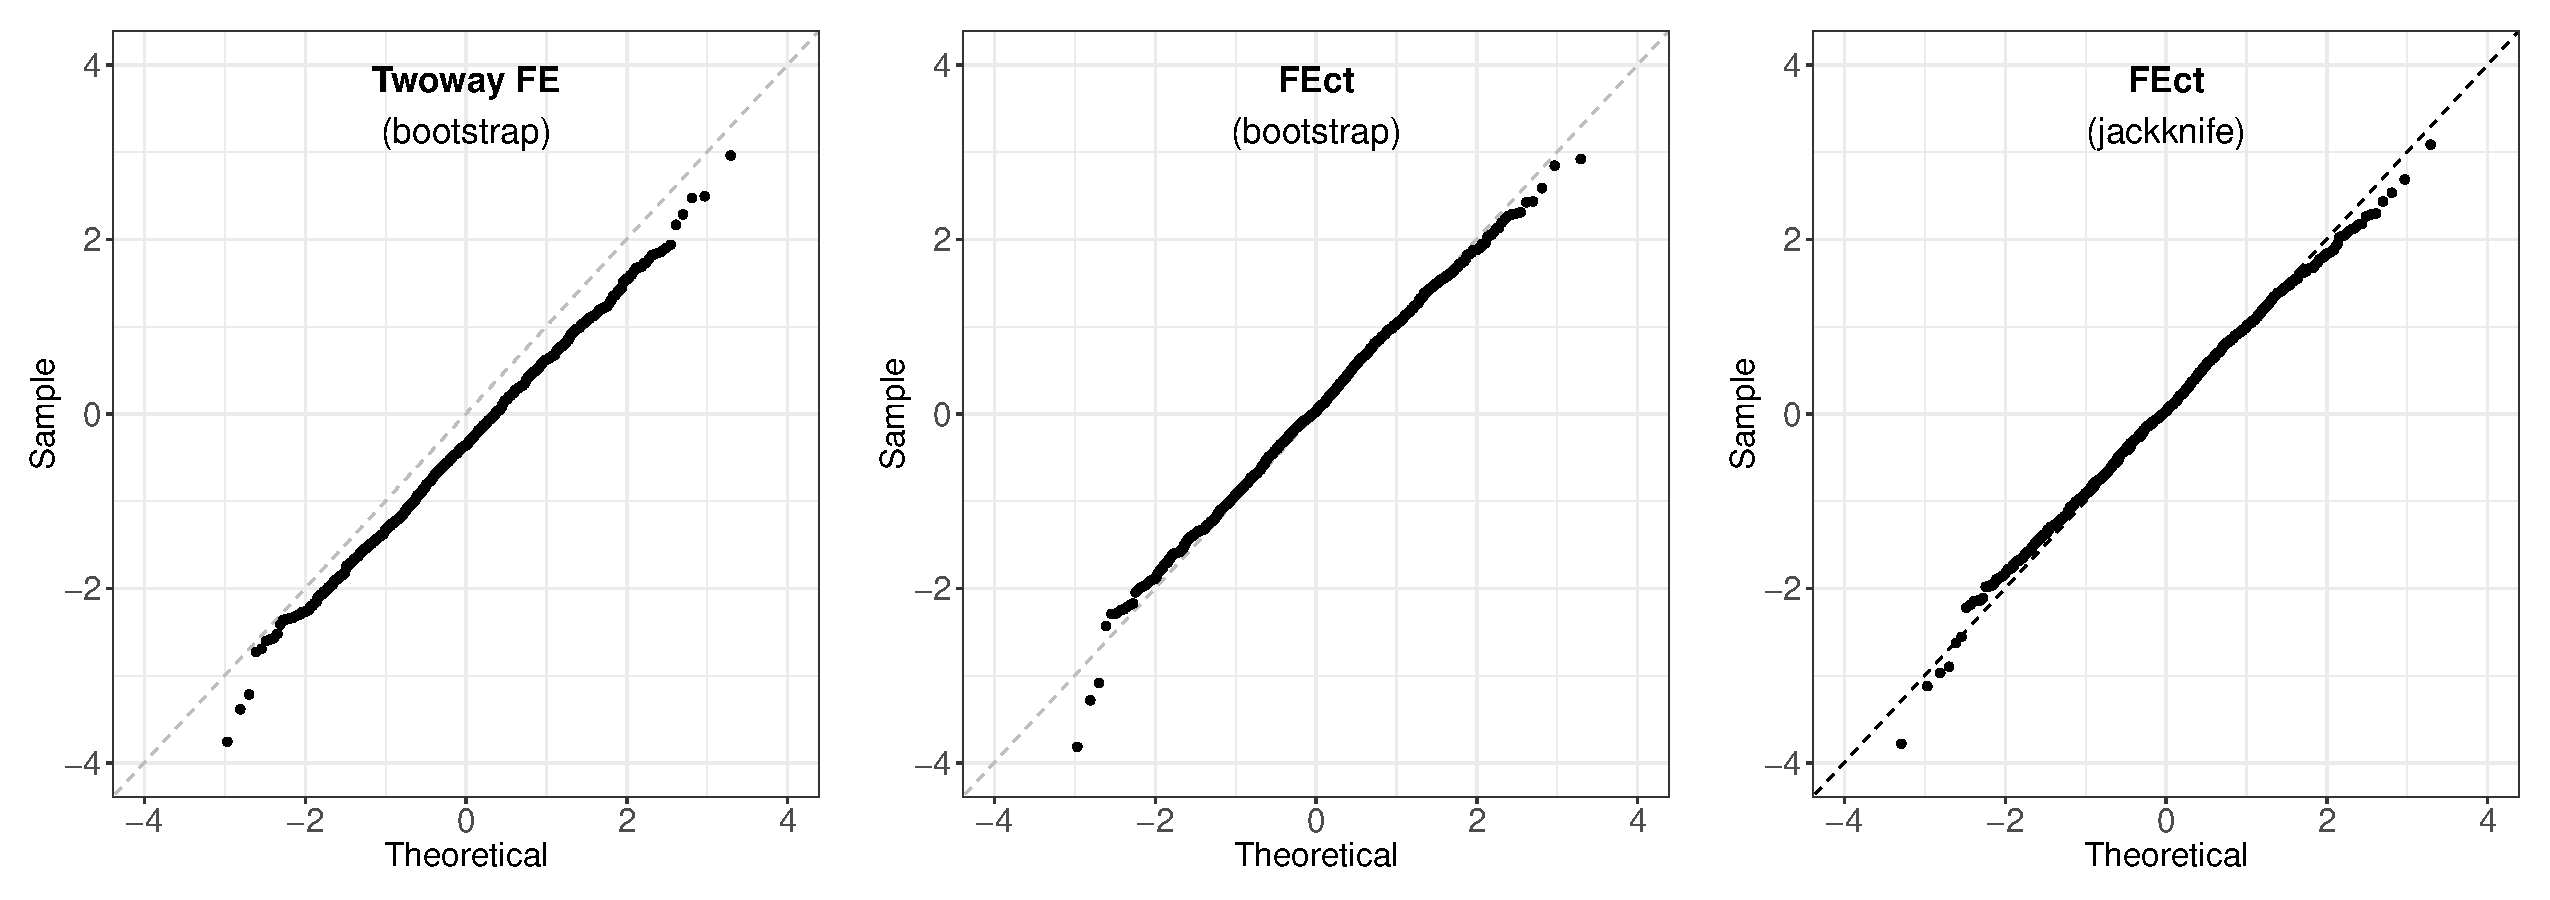
\includegraphics[width = 0.95\textwidth]{sim_infer_n50.pdf}}\\
\subfigure[$N = 100$]{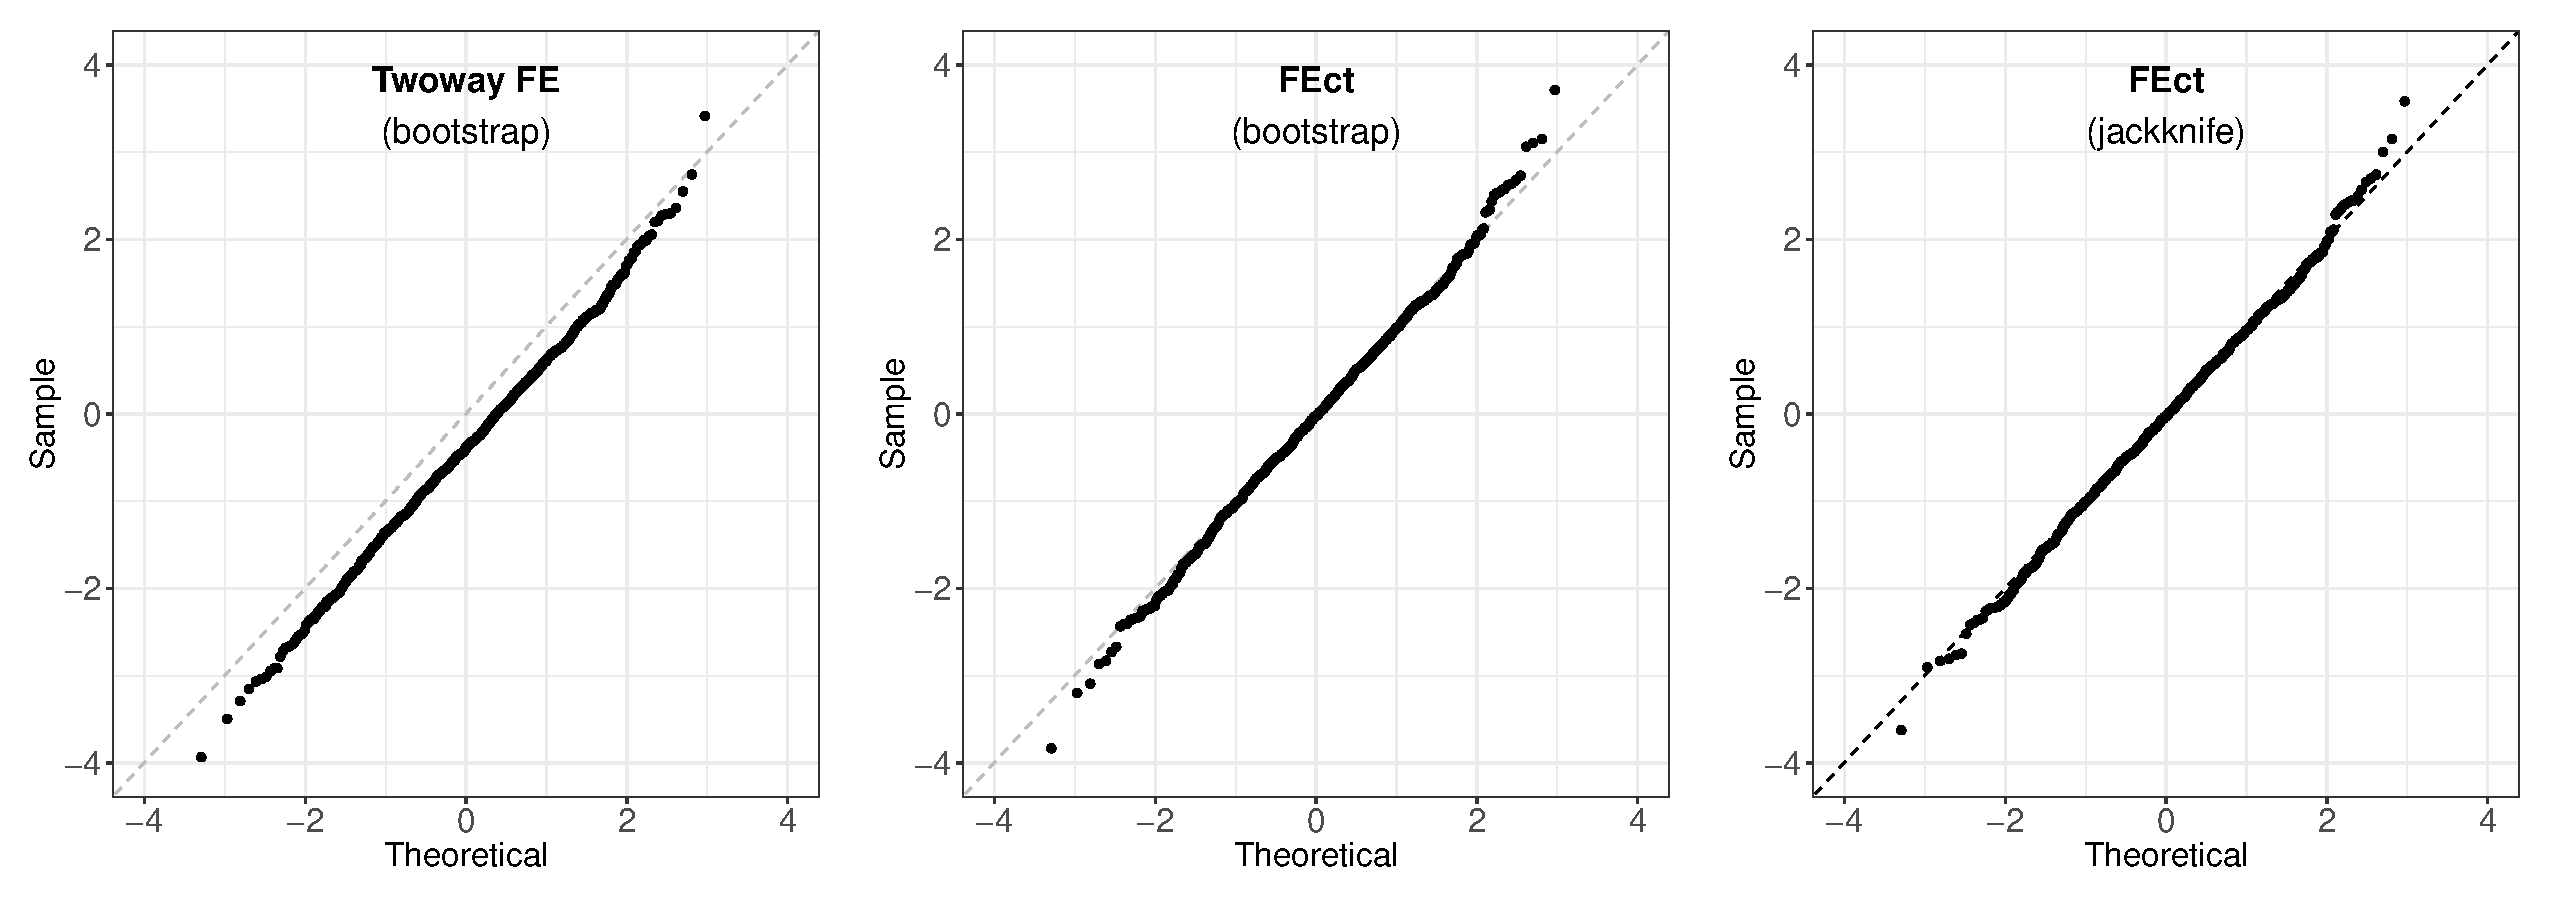
\includegraphics[width = 0.95\textwidth]{sim_infer_n100.pdf}}
\end{center}
\footnotesize\textbf{Note:} The above figures show the standard Gaussian QQ plot of the standardize errors $(\widehat{ATT} - ATT)/(\widehat{\mathrm{Var}}(\widehat{ATT}))^{1/2}$ for the following combination of estimators and inferential methods: (1) twoway fixed effects with block bootstrapped standard errors; (2) FEct with block bootstrapped standard errors; and (3) FEct with jackknife standard errors, each aggregated from 1,000 simulations using samples with dimensions $T = 20$ and $N = 30$, $N = 50$ or $N = 100$. The 45-degree indicates the benchmark: consistent point estimates with perfectly calibrated Gaussian standard errors. 
\end{minipage}
\end{figure}
\clearpage 

\section{Additional Monte Carlo Evidence}\label{sc:sim}

In this section, we report results of three sets of Monte Carlo exercises to demonstrate (1) the finite sample properties of the proposed inferential methods; (2) the differences between the IFEct and MC estimators, and (3) the main advantages of the equivalence test over the $F$ test. Before doing so, we first describe the data generating processes (DGP) of the simulated sample.


\subsection{Describing the DGP of the Simulated Example}

We describe the DGP of the simulated example as follows. 
\begin{itemize}
    \item {\bf Outcome model}: $Y_{it}(0) = \delta_{it} D_{it} + 5 + 1 \cdot X_{it,1} + 3 \cdot X_{it,2} + 1.5 \lambda_{i1}\cdot f_{1t} + \lambda_{i2}\cdot f_{2t}+ \alpha_{i} + \xi_{t} + \varepsilon_{it}$, in which $f_{1t}$ is a linear trend plus a white noise: $f_{1t} = t + \nu_{t}$, and $\nu_{t} \overset{i.i.d}{\sim} N(0,1)$, then it is normalized to have variance 1. $f_{2t}$ is an i.i.d $N(0,1)$ white noise. Both $\lambda_{i1}$ and $\lambda_{i2}$ are i.i.d $N(0,1)$. Two covariates $X_{1,it}$ and $X_{2,it}$ are included in the model. They are both i.i.d. $N(0,1)$. Unit fixed effects $\alpha_{i}\sim N(0,1)$. Time fixed effects $\xi_{t}$ follows a stochastic drift. The error term $\varepsilon_{it}$ is also i.i.d. $N(0,2)$.
    \item {\bf Treatment effects}: $\delta_{it}= 0.4 s_{t} + e_{it}$, in which $s_{t}$ represents the number of periods since the latest treatment's onset and $e_{it}$ is i.i.d. $N(0,0.2^2)$. This means the expected value of the treatment effect gradually increases as a unit takes up the treatment, e.g. from 0.4 in the first period after receiving the treatment to 2.0 in the fifth period. 
    \item {\bf Treatment assignment}: denote $p_{it}$ the probability of getting treated for unit $i$ in period $t$: $logit(p_{it}) = -1 + 0.5 D_{t-1} + 0.5\lambda_{i}'f_{t} + 0.2\alpha_{i} + 0.2\xi_{t} + \mu_{it}$, in which $\mu_{it} \overset{i.i.d}{\sim} N(0,0.1^2)$.
\end{itemize}
Note that this DGP satisfies Assumptions~1-3. Figures~\ref{fg:sim.treat} and \ref{fg:sim.outcome} show the treatment status and outcome variable in the simulated example. 

\begin{figure}[!th]
\caption{Treatment Status: The Simulated Samples}\label{fg:sim.treat}
\centering
\begin{minipage}{0.85\linewidth}{
\begin{center}
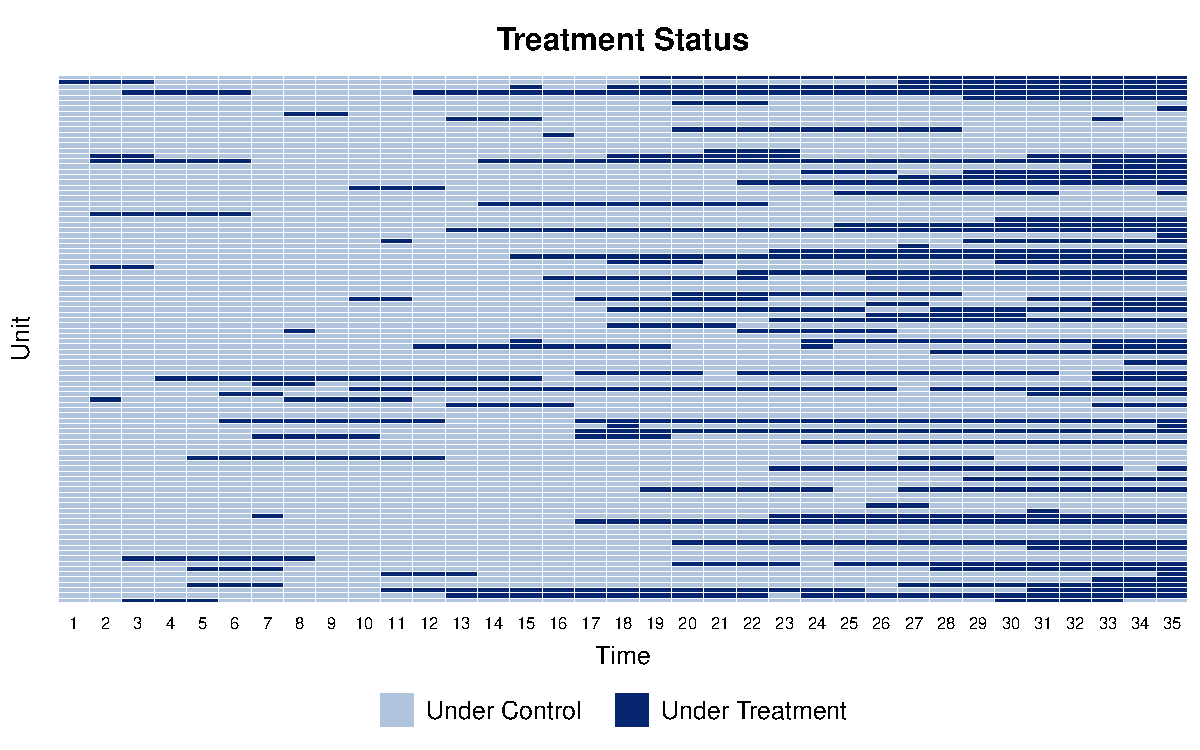
\includegraphics[width = 0.8\textwidth]{sim0_treat.pdf}\\
\end{center}
}
\footnotesize\textbf{Note:} The above figure plots the treatment status of the simulated example, in which treatment reversal is allowed. The plot is made by the \texttt{panelView} package.
\end{minipage}
\end{figure}

\begin{figure}[!th]
\caption{Outcome Variable: The Simulated Samples}\label{fg:sim.outcome}
\centering
\begin{minipage}{0.85\linewidth}{
\begin{center}
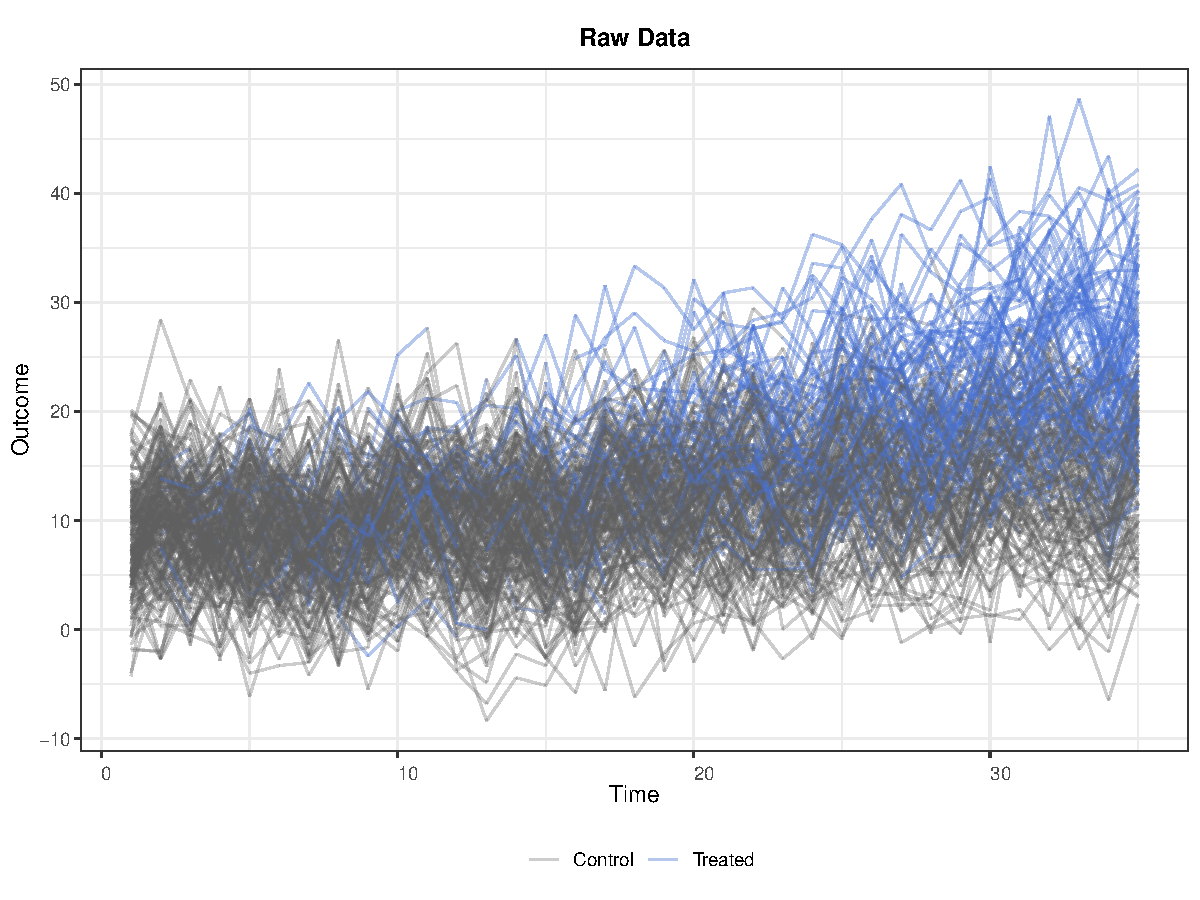
\includegraphics[width = 0.8\textwidth]{sim0_outcome.pdf}\\
\end{center}
}
\footnotesize\textbf{Note:} The above figure plots the outcome variable in the simulated example. The plot is made by the \texttt{panelView} package.
\end{minipage}
\end{figure}
\clearpage




\subsection{IFEct versus MC}

We compare the performance of the IFEct and MC estimators using DGPs similar to that of the simulated example: $Y_{it} = \delta_{it} D_{it} + 5 + \frac{1}{\sqrt{r}}\sum_{m=1}^{r} \lambda_{im} \cdot f_{mt} + \alpha_{i} + \xi_{t} + \varepsilon_{it}.$ We simulate samples of 200 units and 30 time periods, and all treated units receive the treatment at period 21 ($T_{0}= 20$). Following \citet{li2018inference}, we vary the number of factors $r$ from 1 to 9 and adjust a scaling parameter $\frac{1}{\sqrt{r}}$ such that the total contribution of all factors (and their loadings) to the variance of $Y$ remains constant. Our intuition is that IFEct (i.e., hard impute) performs better than MC (i.e., soft impute) when only a small number of factors are present and each of them exhibits relatively strong signals while MC outperforms IFEct when a large set of weak factors exist. In other words, MC should handle sparsely distributed factors better than parametric models like IFEct. 
\begin{figure}[!ht]
\caption{Monte Carlo Exercises: IFEct vs. MC}\label{fg:sim.estimators}
\centering
\begin{minipage}{0.95\linewidth}
\begin{center}
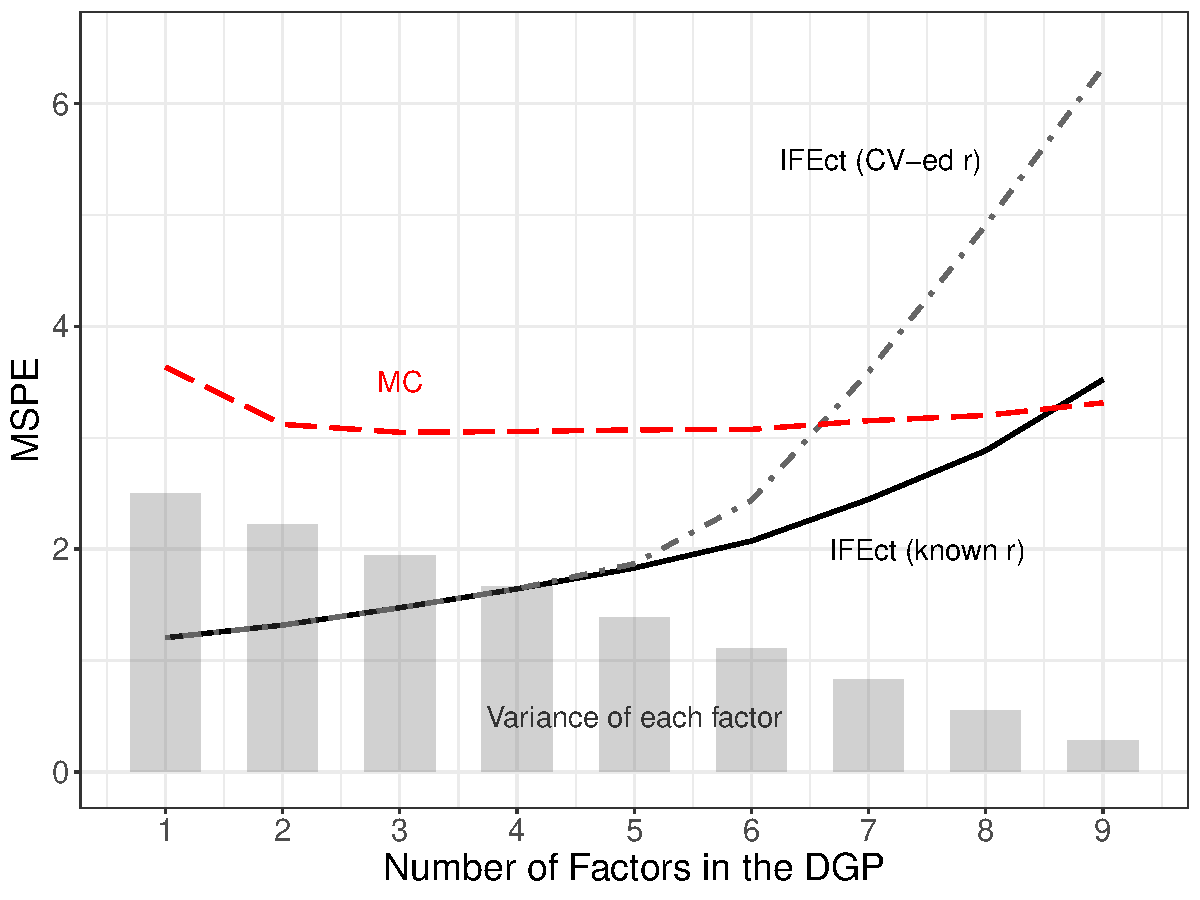
\includegraphics[width = 0.8\textwidth]{sim_compare.pdf}
\end{center}
\footnotesize\textbf{Note:} The above figure compares the mean squared prediction errors (MSPEs) for treated counterfactuals using the IFEct and MC estimators with different DGPs in which the total variance of all factors are kept constant. 
\end{minipage}
\end{figure}

The results are shown in Figure~\ref{fg:sim.estimators}, which depicts the MSPE of treated counterfactuals, i.e., $\frac{1}{\#\mathbf{1}\{(i,t)| D_{it}=1\}}\sum_{D_{it} = 1} [Y(0) - \hat{Y}_{it}(0)]^{2}$ , from 500 simulations using these two methods. The black solid line and gray dashed line represent the MSPE of IFEct with the correct number of factors ($r$) and with cross-validated $r$'s, respectively, while the red dot-dashed line marks the MSPEs of the MC estimator with a crossed validated tuning parameter $\lambda$. The result shows that MC gradually catches up with, and eventually beats, IFEct (with correctly specified $r$) as the number of factor grows and each factor produces weaker signals. It also suggests that, when factors become weaker, it is more difficult for the cross-validation scheme to pick them up, resulting in worse predictive performance, while the MC estimator is robust to a large number of factors because factors and loadings are not directly estimated. 
\bigskip

\subsection{$F$ Test versus the Equivalence test.} 

As explained in the paper, there is a trade-off between the $F$ test and the equivalence test (TOST) for testing no pre-trend: (1) when the sample size is small, the $F$ test has a power issue while TOST does not; and (2) when the sample size is relatively large, TOST are more liberal than the $F$ test in front of small biases. To illustrate these, we simulate data using the following DGP similar to that in the previous section but with only one factor: $Y_{it} = \delta_{it} D_{it} + 5 + k \cdot \lambda_{i}  f_{t} + \alpha_{i} + \xi_{t} + \varepsilon_{it},$ in which we vary $k$ to adjust the influence of a potential confounder $U_{it} = \lambda_{i} f_{t}$, which is correlated with $D_{it}$. For each $k$, we run 600 simulations. In each simulation, we first generate a sample of $N = 100$ units (50 treated and 50 controls) of 40 periods. We estimate a FEct model without taking into account the time-varying confounder. We then expand the sample size such that $N = 300$ and re-do the analysis.

In Figure~\ref{fg:sim.tests}(a), we plot the proportion of times the equivalence test (solid line) or the $F$ test (dashed line) backs the strict exogeneity assumption against the normalized bias induced by the confounder when $N = 100$. It shows that it is highly likely that an $F $test cannot reject the null of zero residual average due to lack of power, even when the biases are large. In contrast, the probability that the equivalence test rejects inequivalence (hence, declaring equivalence) drops quickly as the bias increases. In other words, the equivalence test is more powerful in detecting imbalances than the conventional $F$ test. Figure~\ref{fg:sim.tests}(b) shows that, when the sample size is relatively large ($N = 300$), the non-rejection rate of the $F$ test declines quickly as the influence of the confounder grows. In comparison, the equivalence test rejects inequivalence (hence, declaring equivalence) when a relatively inconsequential confounder is at present; as the confounder becomes more influential, it starts to sound the alarm. These patterns are similar to what \citet{hartman2018equivalence} report in a cross-sectional setting. 
\clearpage

\begin{figure}[!ht]
\caption{Monte Carlo Exercises: $F$ vs. equivalence tests}\label{fg:sim.tests}
\begin{center}
\hspace{-1em}
\subfigure[$N = 100$]{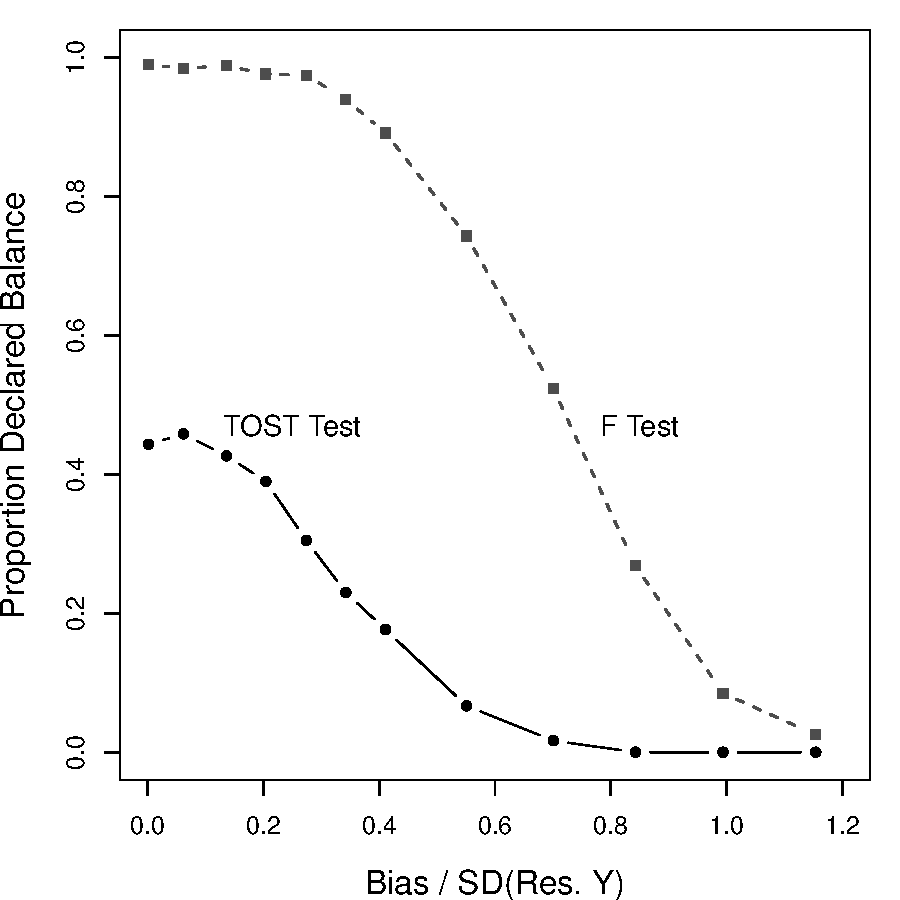
\includegraphics[width = 0.45\textwidth]{sim_tests_n100.pdf}}\hspace{0.5em}
\subfigure[$N = 300$]{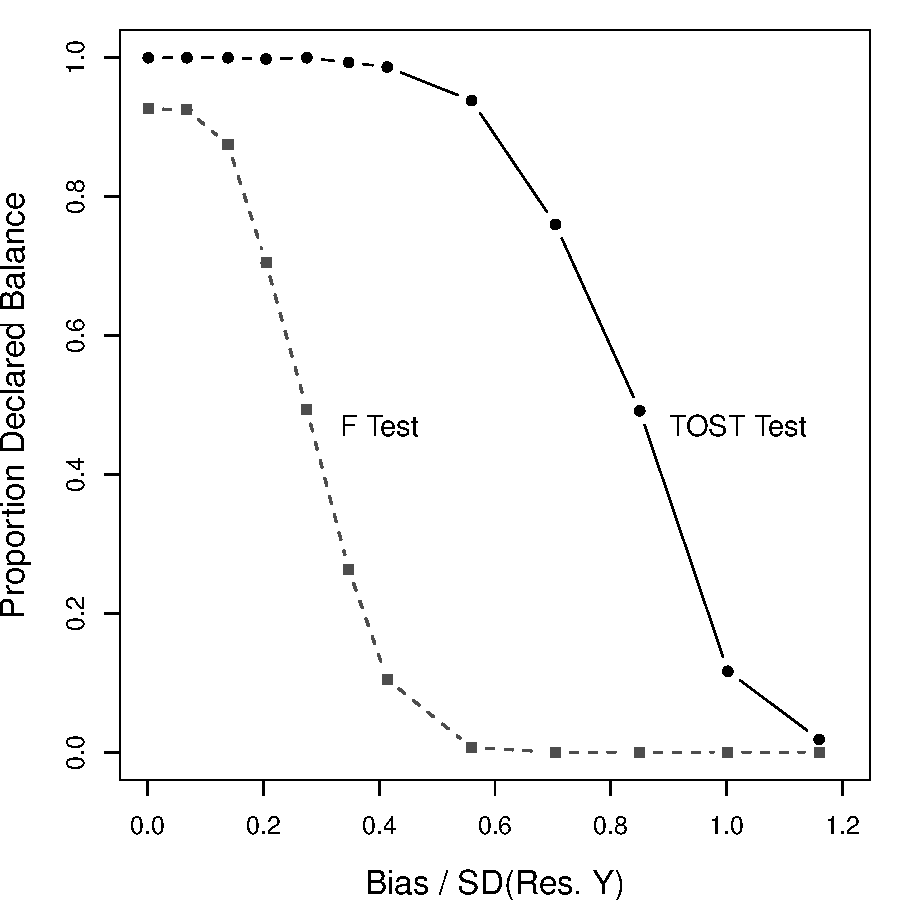
\includegraphics[width = 0.45\textwidth]{sim_tests_n300.pdf}}\hspace{0.5em}
\end{center}
\footnotesize\textbf{Note:} The above figures show the results from Monte Carlo exercises that compare the $F$ test and the equivalence test when an unobserved confounder exists. In plot (a), $N = 100$; in plot (b), $N = 300$. Each dot is based on results from 600 simulations. 
\end{figure}

\clearpage

% Figure~\ref{fg:sim.tests}(b) and (c) show how the performances of the two tests change as the number of units $N$ increases under two circumstances: when the bias induced by the confounder is relatively small ($0.10\sigma_{Y}$) and when the bias is relatively large ($0.28\sigma_{Y}$). The results suggest that in both scenarios, the $F$ test is more likely rejects the null (hence, declaring inequivalence) as the sample size grows while the equivalence test behaves differently: when the bias is small, the probability of declaring equivalence grows with sample size and stays high; when the bias is large, the probability of declaring equivalence decreases with the sample size. The equivalence test has more desirable properties because it tolerates inconsequential confounders  but is capable of detecting ones that cause large biases. 



%%%%%%%%%%%%%%%%%%%%%%%%%%%%%%%%%%%%%%%%%%%%%%%%%%%%%%%
%%%%%%%%%%%%%%%%%%%%%%%%%%%%%%%%%%%%%%%%%%%%%%%%%%%%%%%
%%%%%%%%%%%%%%%%%%%%%%%%%%%%%%%%%%%%%%%%%%%%%%%%%%%%%%%
%%%%%%%%%%%%%%%%%%%%%%%%%%%%%%%%%%%%%%%%%%%%%%%%%%%%%%%
%%%%%%%%%%%%%%%%%%%%%%%%%%%%%%%%%%%%%%%%%%%%%%%%%%%%%%%
%%%%%%%%%%%%%%%%%%%%%%%%%%%%%%%%%%%%%%%%%%%%%%%%%%%%%%%
%%%%%%%%%%%%%%%%%%%%%%%%%%%%%%%%%%%%%%%%%%%%%%%%%%%%%%%
%%%%%%%%%%%%%%%%%%%%%%%%%%%%%%%%%%%%%%%%%%%%%%%%%%%%%%%
%%%%%%%%%%%%%%%%%%%%%%%%%%%%%%%%%%%%%%%%%%%%%%%%%%%%%%%
%%%%%%%%%%%%%%%%%%%%%%%%%%%%%%%%%%%%%%%%%%%%%%%%%%%%%%%
%%%%%%%%%%%%%%%%%%%%%%%%%%%%%%%%%%%%%%%%%%%%%%%%%%%%%%%
%%%%%%%%%%%%%%%%%%%%%%%%%%%%%%%%%%%%%%%%%%%%%%%%%%%%%%%
%%%%%%%%%%%%%%%%%%%%%%%%%%%%%%%%%%%%%%%%%%%%%%%%%%%%%%%

\section{Additional Information on the Empirical Examples}

\subsection{Replicating Hainmueller and Hangartner (2015)}

\begin{figure}[!th]
\caption{Treatment Status: Indirect Democracy and\\Naturalization Rate}\label{fg:XY2015}
\centering
\begin{minipage}{0.85\linewidth}{
\begin{center}
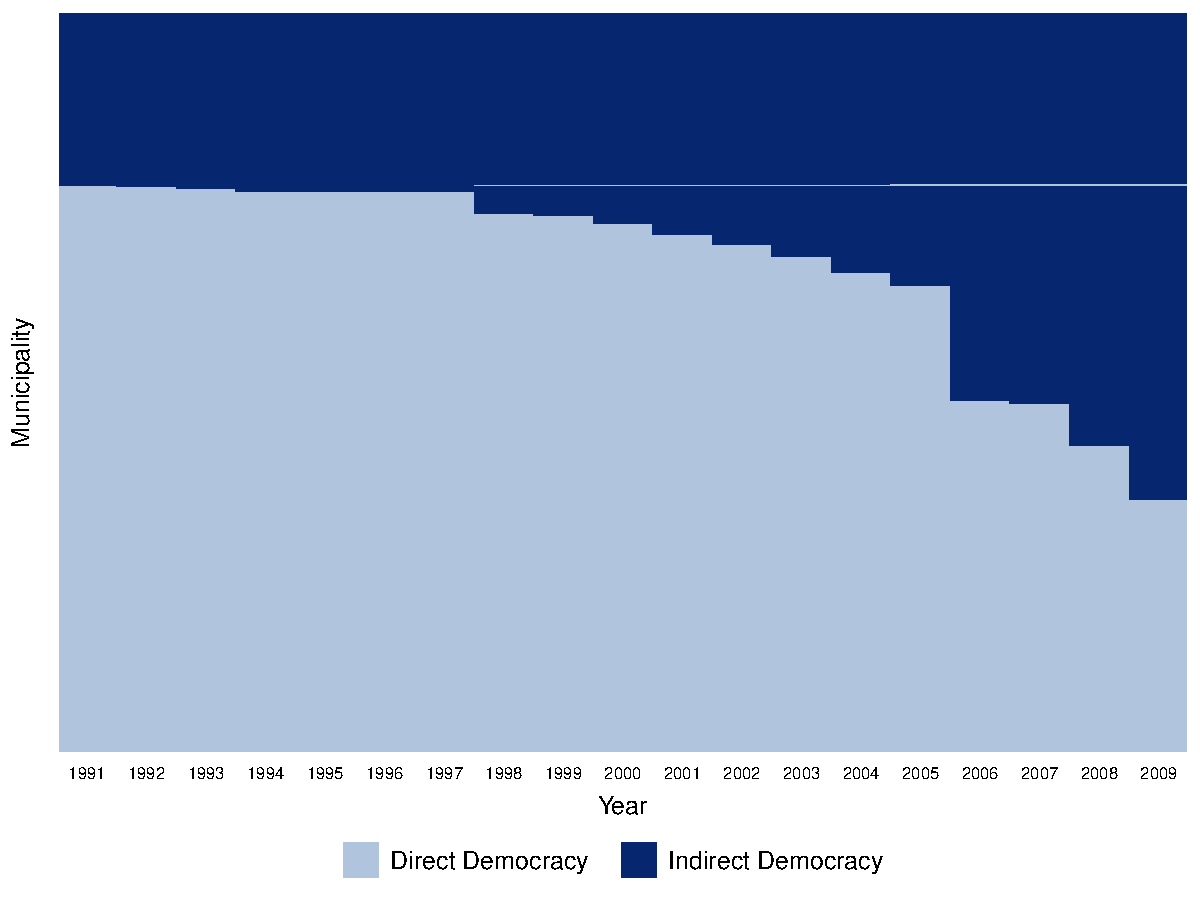
\includegraphics[width = 0.8\textwidth]{ex_HH2015_treat.pdf}\\
\end{center}
}
\footnotesize\textbf{Note:} The above figure plots the treatment status for the first 50 units using data from \citet{hainmueller2015does}. The pattern of treatment assignment follows staggered adoption. Municipalities are ordered based on the timing when they started to adopt indirect democracy to make naturalization decisions. The plot is made by the \texttt{panelView} package.
\end{minipage}
\end{figure}

\clearpage

\subsection{Replicating Fouirnaies and Mutlu-Eren (2015)}

\begin{figure}[!th]
\caption{Original Treatment Effect Plot}\label{fg:FM2015.original}
\centering
\begin{minipage}{1\linewidth}{
\begin{center}
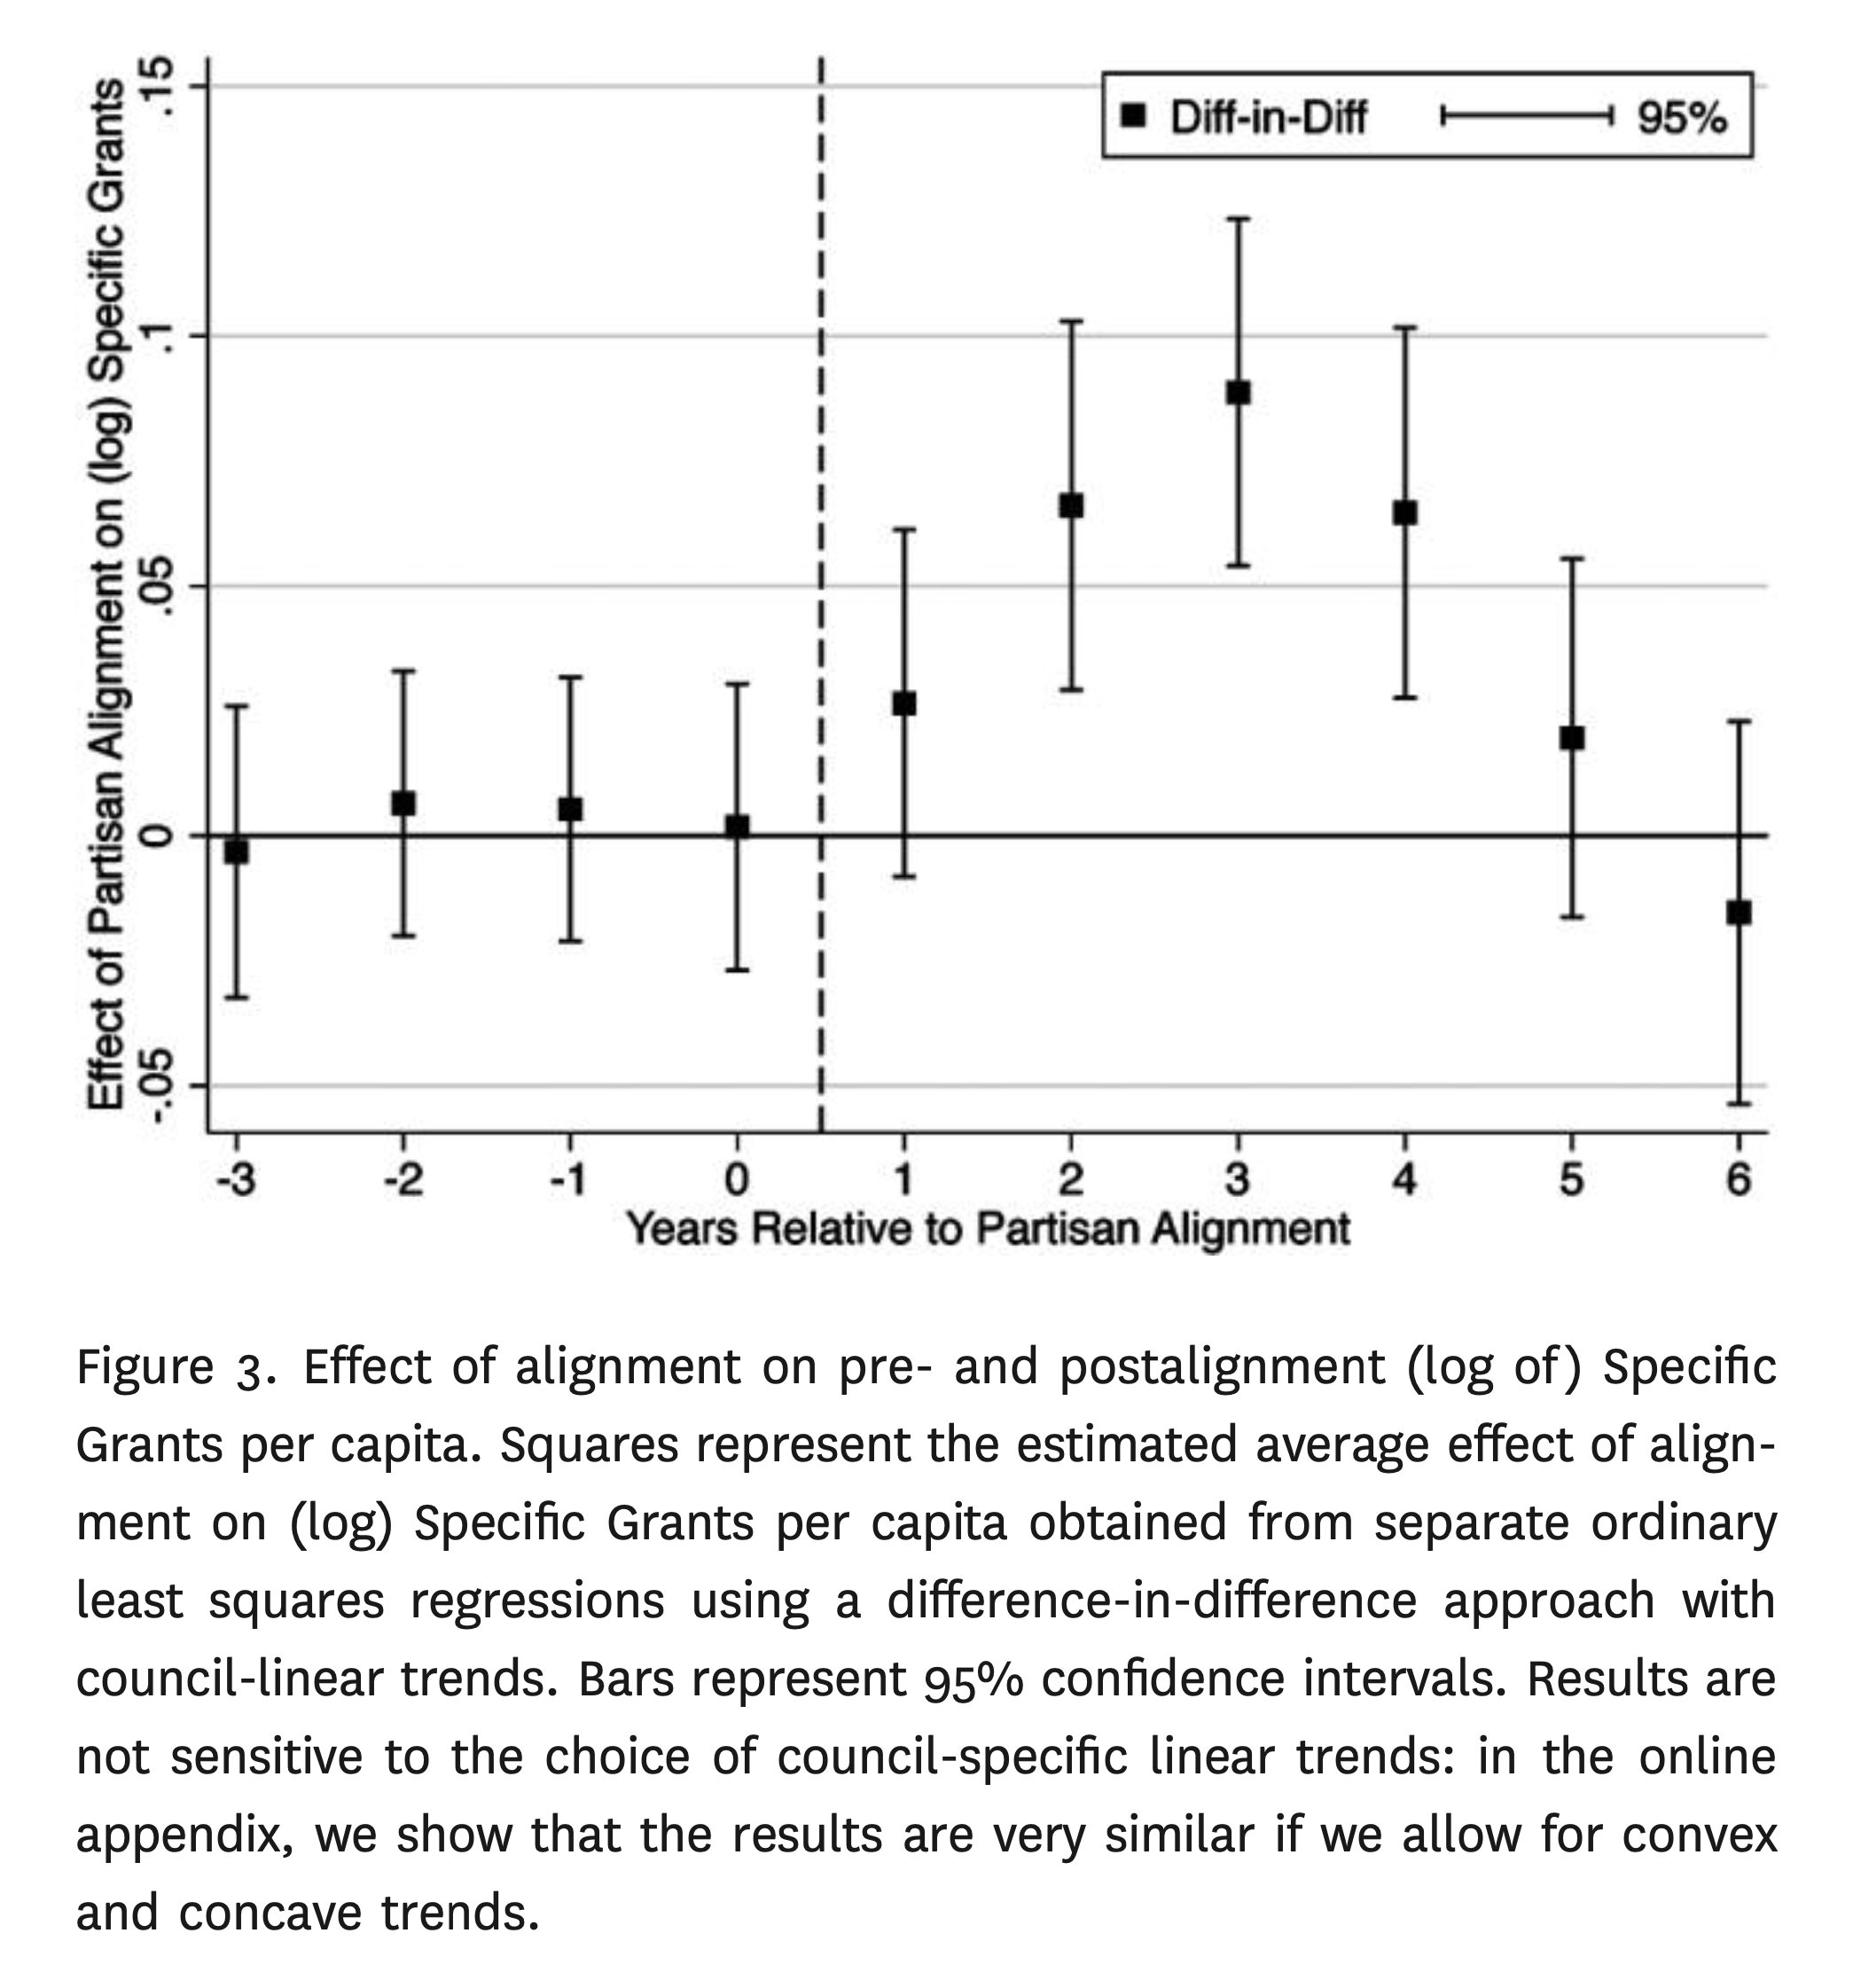
\includegraphics[width = 0.75\textwidth]{ex_FM2015_fig3.png}\\
\footnotesize\textbf{Note:} The above figure is adapted from \citet{FM2015-yy}.
\end{center}
} 
\end{minipage}
\end{figure}
\clearpage

\begin{figure}[!th]
\caption{Treatment Status: Partisan Alignment and Specific Grants}\label{fg:FM2015.treat}
\centering
\begin{minipage}{1\linewidth}{
\begin{center}
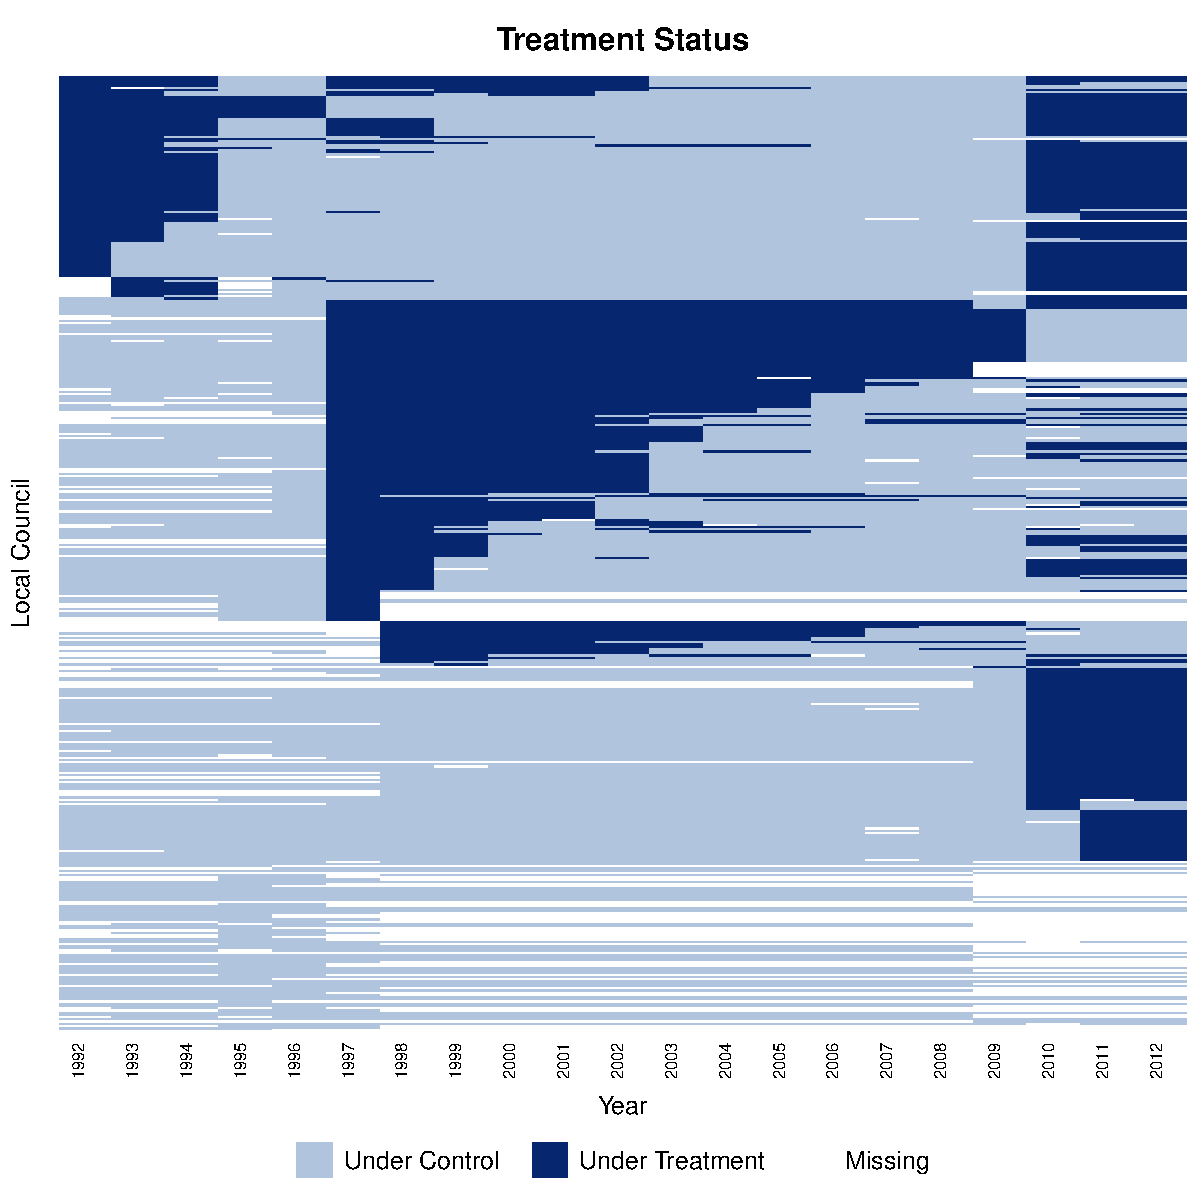
\includegraphics[width = 0.55\textwidth]{ex_FM2015_treat.pdf}
\end{center}
}
\footnotesize\textbf{Note:} The above figure plots the treatment status  using data from \citet{FM2015-yy}. Local councils in England are ordered based on the timing when they are politically aligned with the government party. The plot is made by the \texttt{panelView} package.
\end{minipage}
\end{figure}


\begin{figure}[!ht]
\caption{The Effect of Partisan Alignment on Specific Grants\\Testing No Pre-Trend}\label{fg:FM2015.equiv}
\centering
\begin{minipage}{1\linewidth}{
\centering
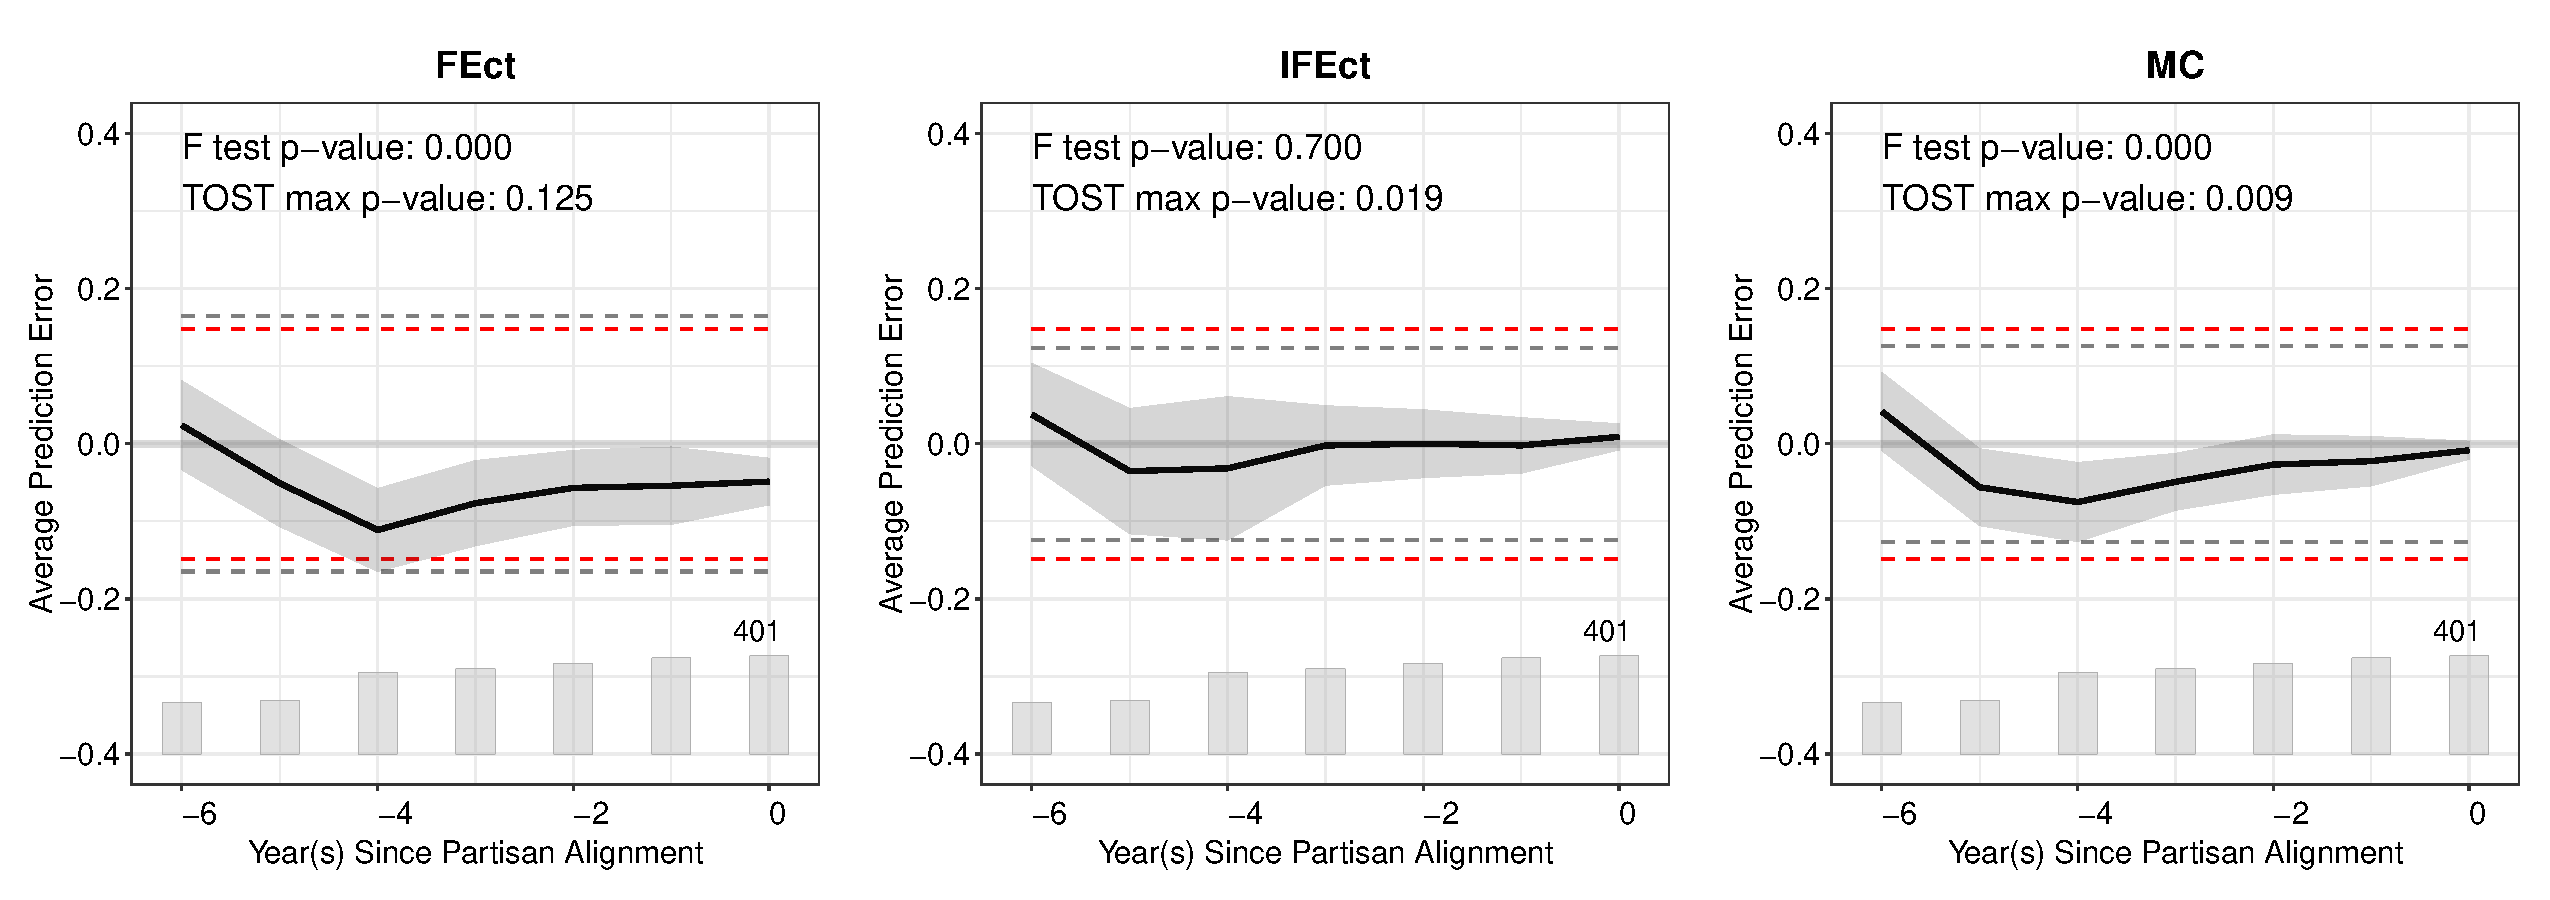
\includegraphics[width = 1\textwidth]{ex_FM2015_equiv.pdf}}
\footnotesize\textbf{Note:} The above figures show the results from tests for no pre-trend in the application of partisan alignment on specific grants in the UK. The bar plot at the bottom of each figure illustrates the number of treated units at a given time period relative to the onset of the treatment. Pretreatment residual averages and their 90\% confidence intervals are drawn; the red and gray dashed lines mark the equivalence range and the minimum range, respectively. With the equivalence threshold set at $0.36\hat\sigma^2$, all three models pass the equivalence test. 
\end{minipage}
\end{figure}
\clearpage


\begin{figure}[!ht]
\caption{The Effect of Partisan Alignment on Grant Allocation\\Three Years after the Treatment Ends as the ``Carryover Period''}\label{fg:FM2015b}
\centering
\begin{minipage}{0.9\linewidth}{
\centering
\subfigure[Dynamic Treatment Effects]{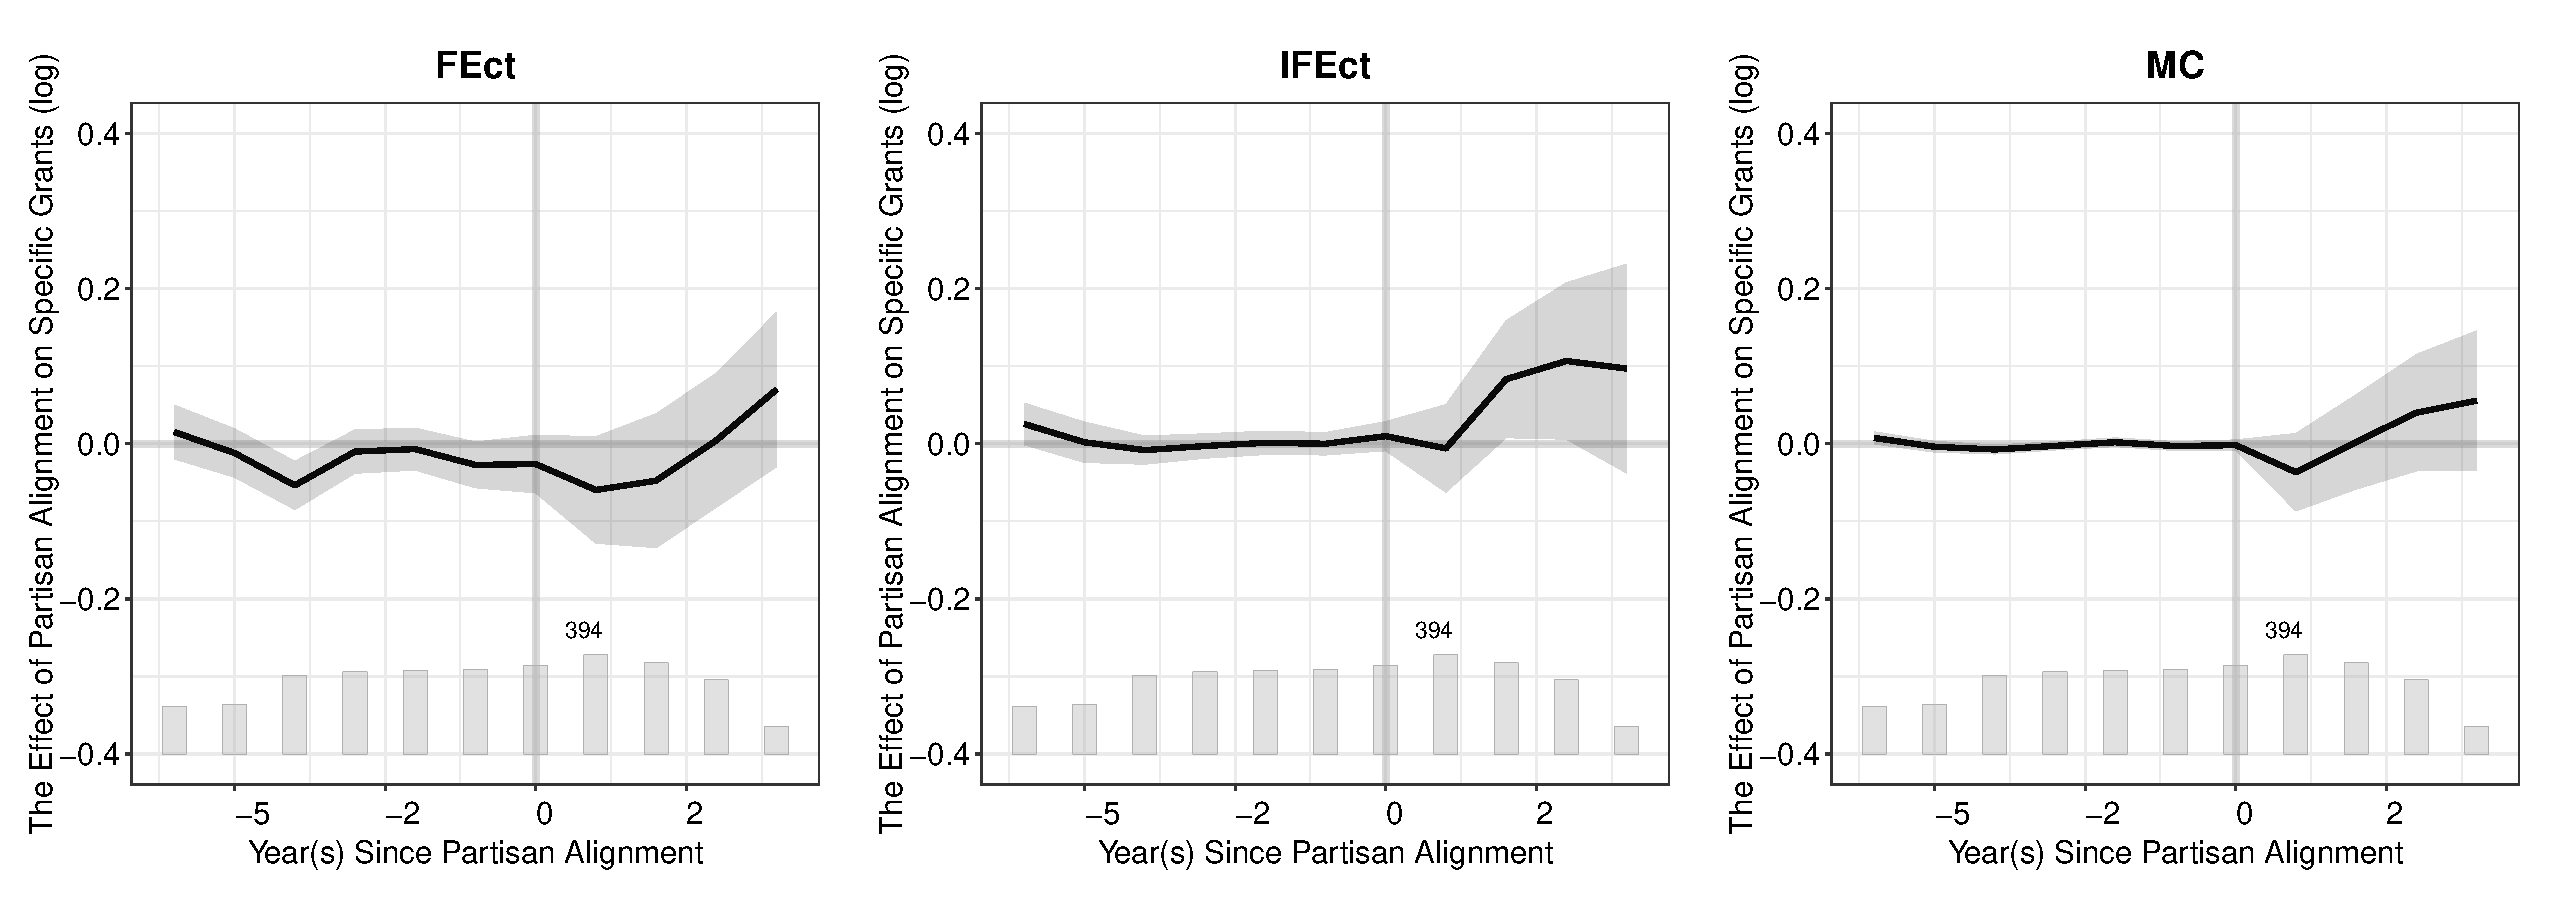
\includegraphics[width = 1\textwidth]{ex_FM2015b_gap.pdf}}\\
\subfigure[Placebo Test]{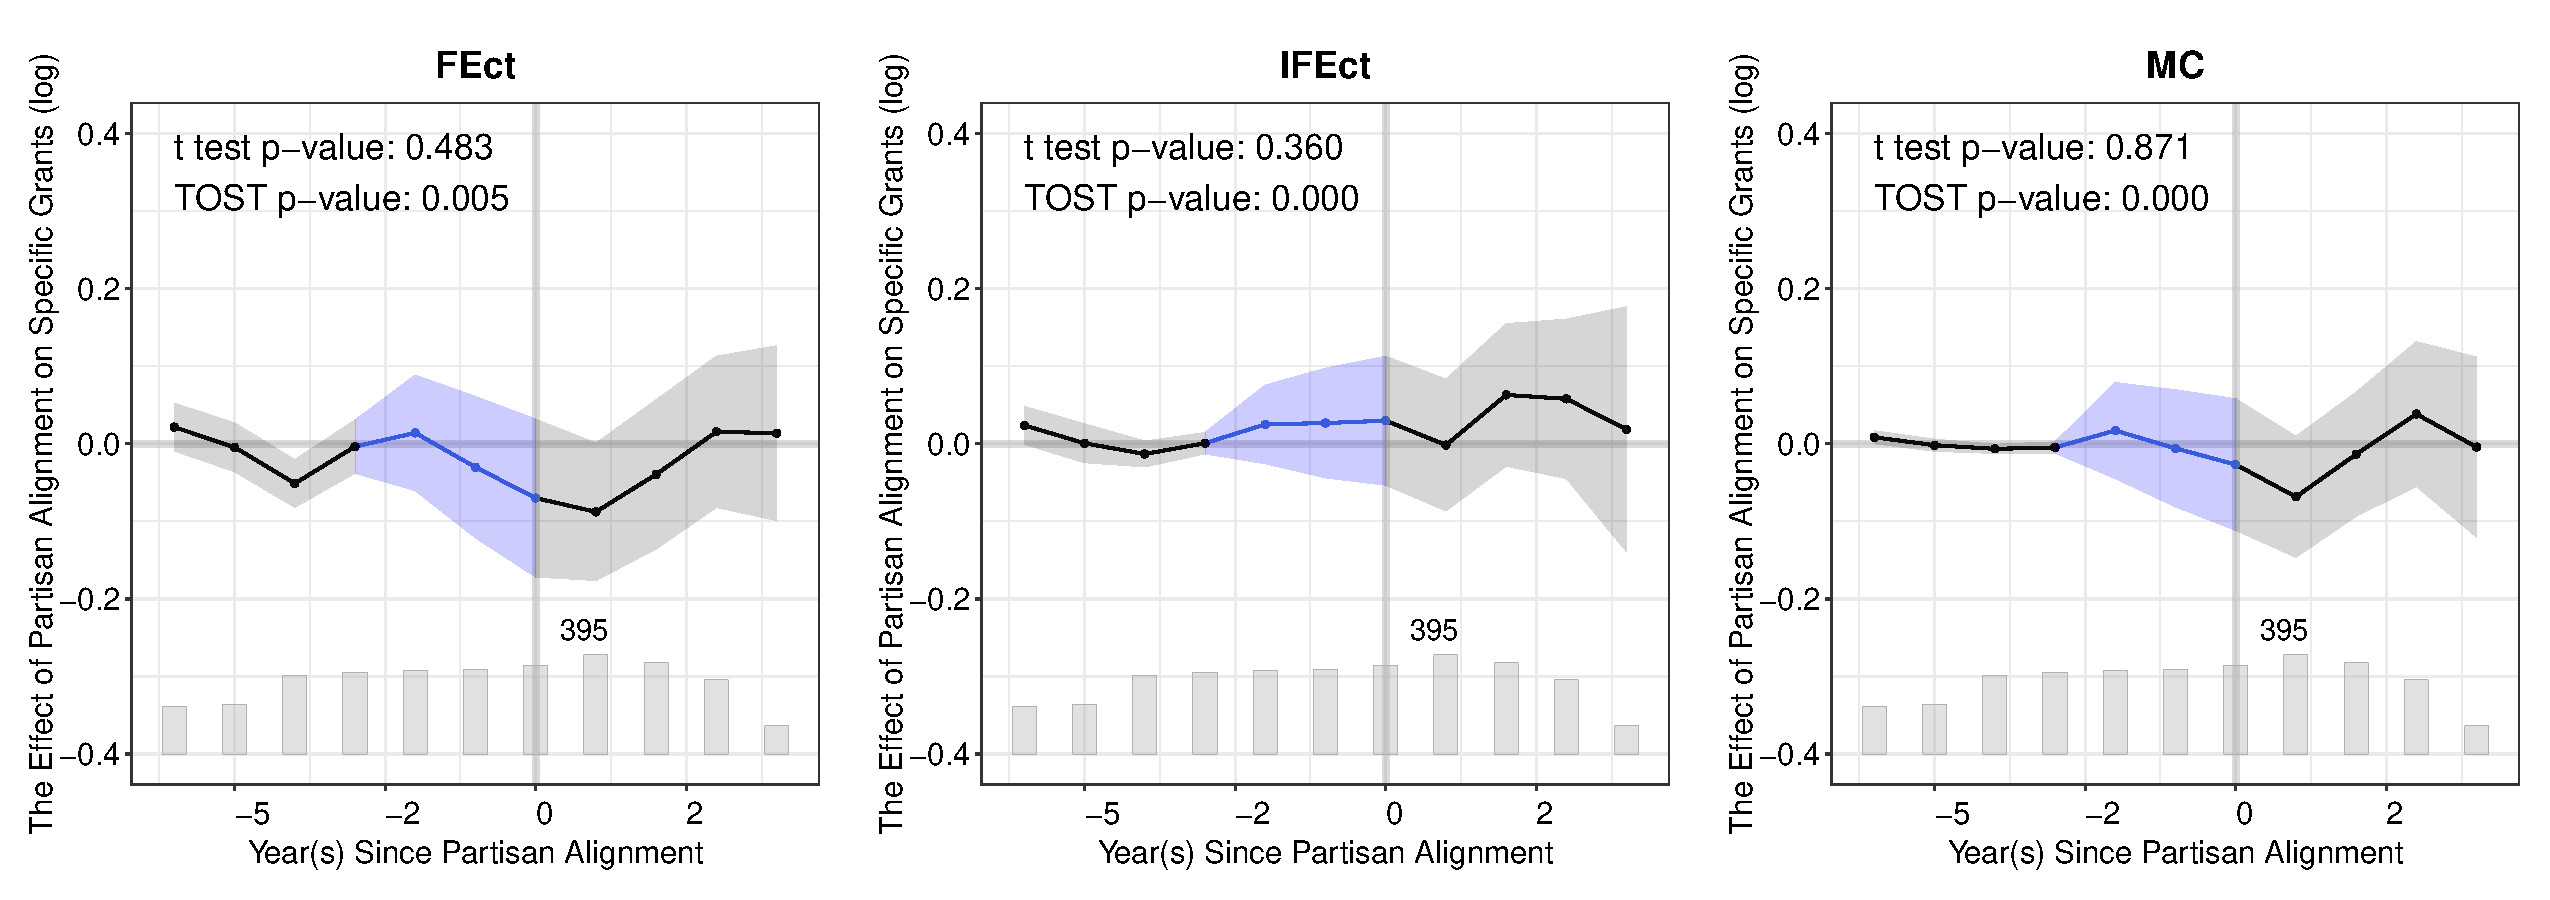
\includegraphics[width = 1\textwidth]{ex_FM2015b_placebo.pdf}}
\subfigure[Test for Carryover Effects]{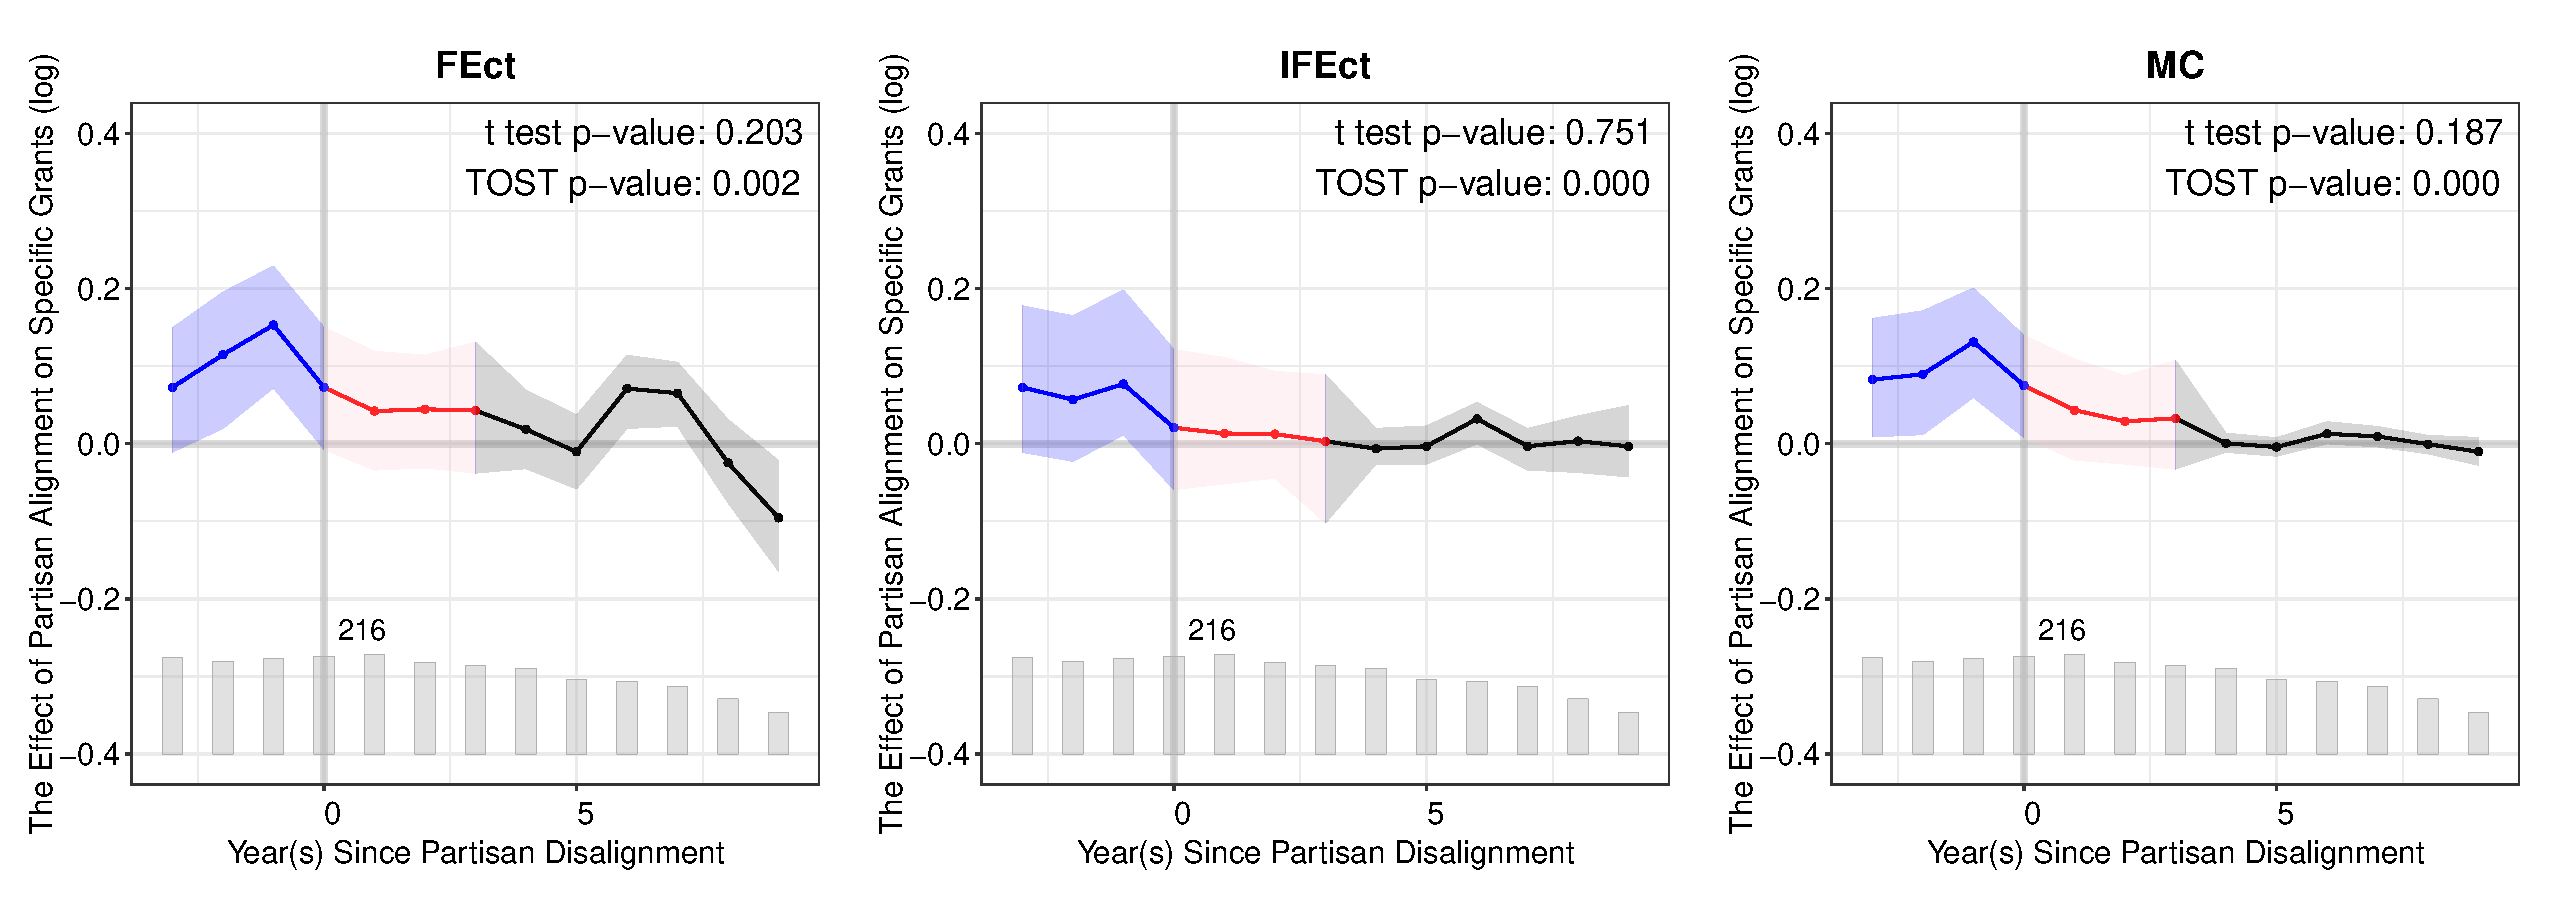
\includegraphics[width = 1\textwidth]{ex_FM2015b_carryover.pdf}}
}
\footnotesize\textbf{Note:} The blue dots in (b) represent the periods used in the placebo tests. In (c), the blue and red dots represent the periods removed from the model-modeling stage (Step 1) and the periods used in the tests for no carryover effects, respectively. 
\end{minipage}
\end{figure}
\clearpage

\begin{figure}[!ht]
\caption{The Effect of Partisan Alignment on Specific Grants:\\by Cohort}\label{fg:FM2015.cohort}
\centering
\begin{minipage}{1\linewidth}{
\centering
\subfigure[FEct]{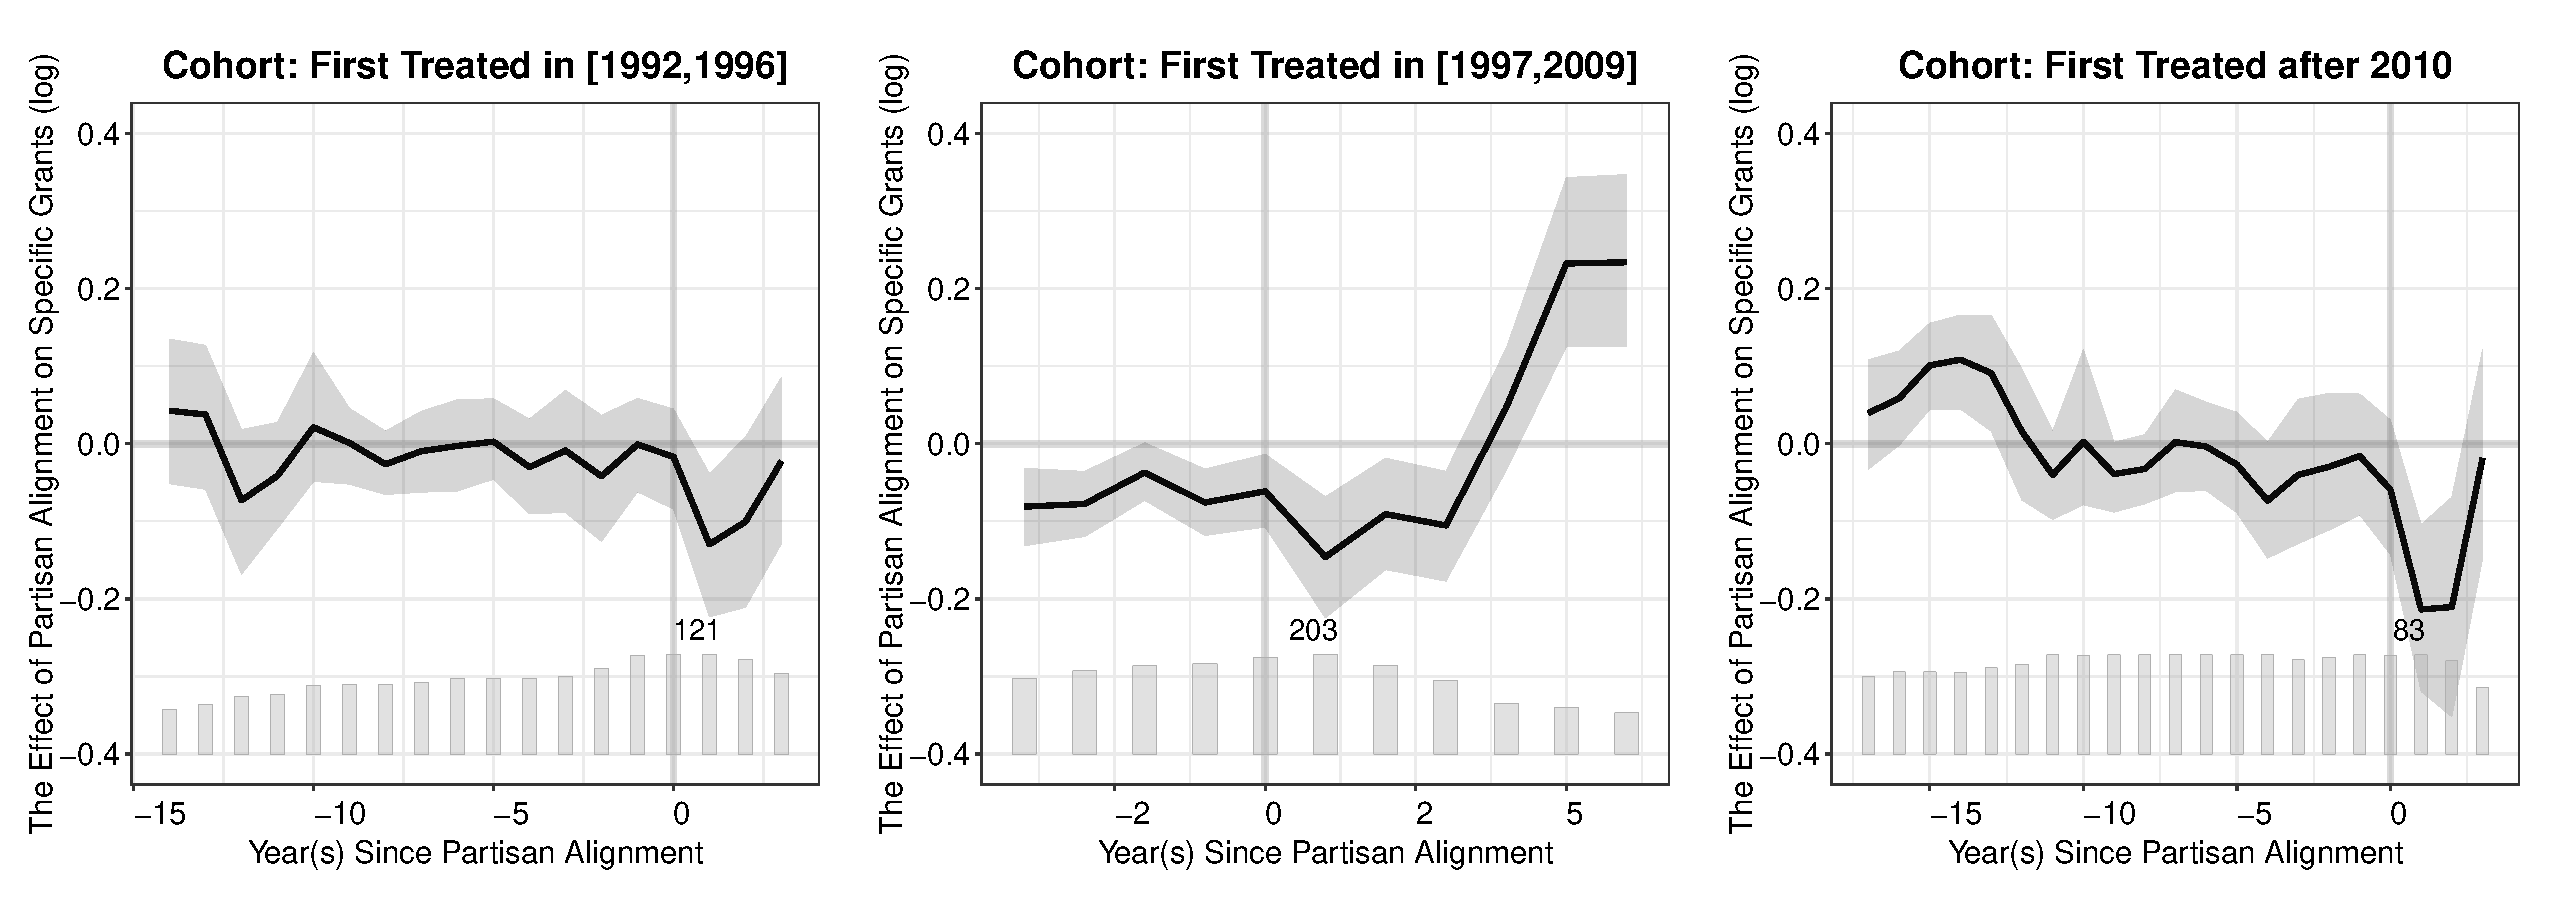
\includegraphics[width = 1\textwidth]{ex_FM2015_cohorts0.pdf}}
\subfigure[IFEct]{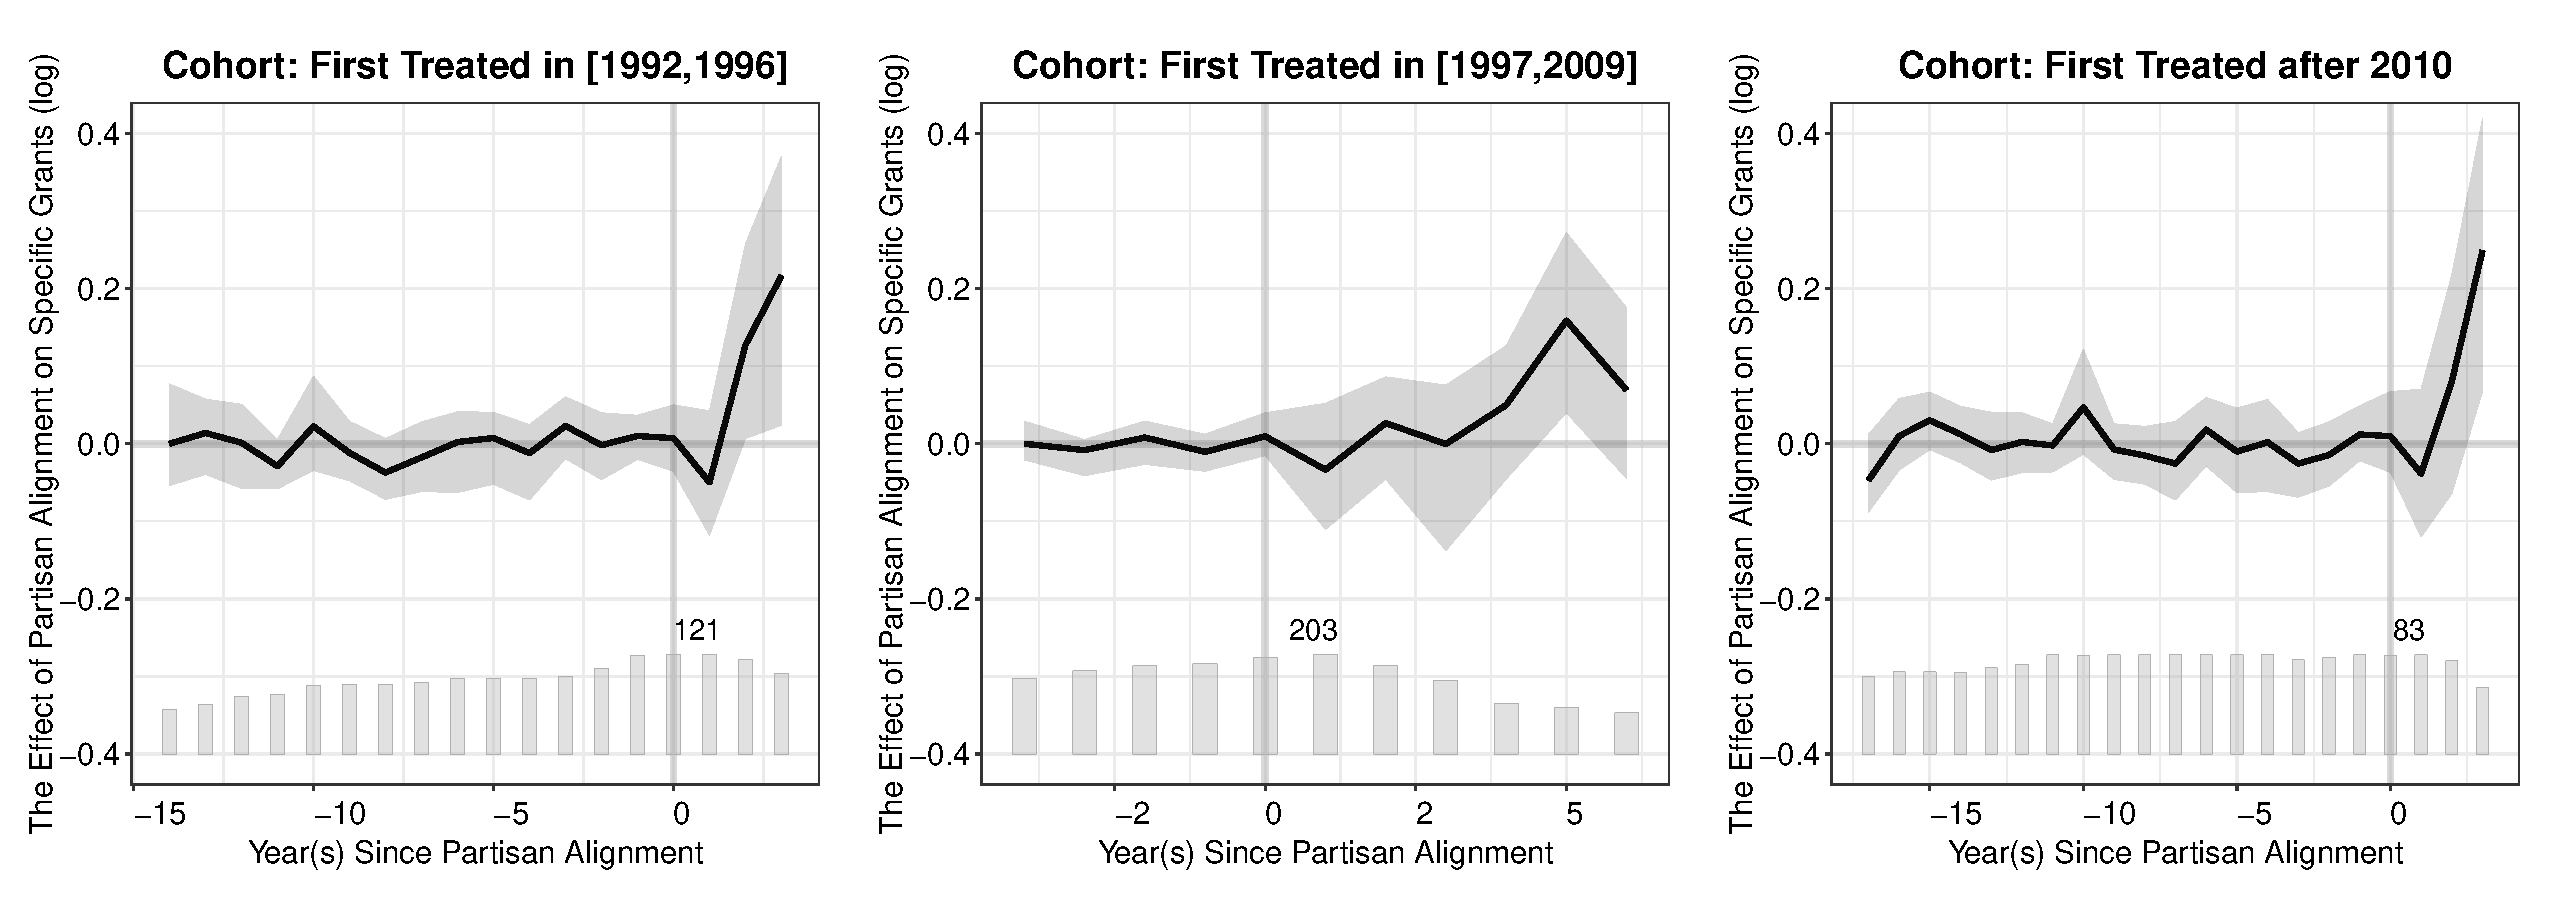
\includegraphics[width = 1\textwidth]{ex_FM2015_cohorts.pdf}}}
\footnotesize\textbf{Note:} The above figures show the effect of partisan alignment on specific grants using FEct (a) and IFEct (b). Cohorts are defined based on the timing when a local council in England is first aligned with the government party. They broadly correspond to the three blocks of units in the treatment status plot (Figure~\ref{fg:FM2015.treat}).
\end{minipage}
\end{figure}
\clearpage


\newpage



\bibliographystyle{apsr}
\bibliography{tscs}

\end{document}

